%! TEX program = LuaTeX

\documentclass[nobackground,dvipsnames,table]{beamer}
\usepackage{cs152}

\mode<presentation>
{\usetheme{Hannover}
    \usecolortheme{cs152}
    \setbeamercovered{transparent}
    \useinnertheme[shadow=false]{rounded}
    \usebackgroundtemplate{}
    \setbeamercolor*{frametitle}{parent=palette primary}
    \setbeamerfont{block title}{size={}}
    \setbeamertemplate{navigation symbols}{}
}

\title{Harassment, Bullying and Threatening Behavior}
\subtitle{CS 152 --- Trust and Safety Engineering}

\author[A. Stamos]{Alex Stamos}
\institute[Stanford University]{Stanford Cyber Policy Center}
\date[2022]{\today}
\subject{CS 152 --- Trust and Safety Engineering}
%\titlegraphic{
\includegraphics[width=5cm]{img/cyber-logo-white-black-red-WEB}}

% Change the level of bulleting on the ToC page
\setcounter{tocdepth}{2}

\graphicspath{{img/lesson06}}

\begin{document}

\begin{frame}
    \titlepage
\end{frame}

\begin{frame}{}%TODO3 Formatting
    \thispagestyle{empty}
    \AddToShipoutPictureBG*{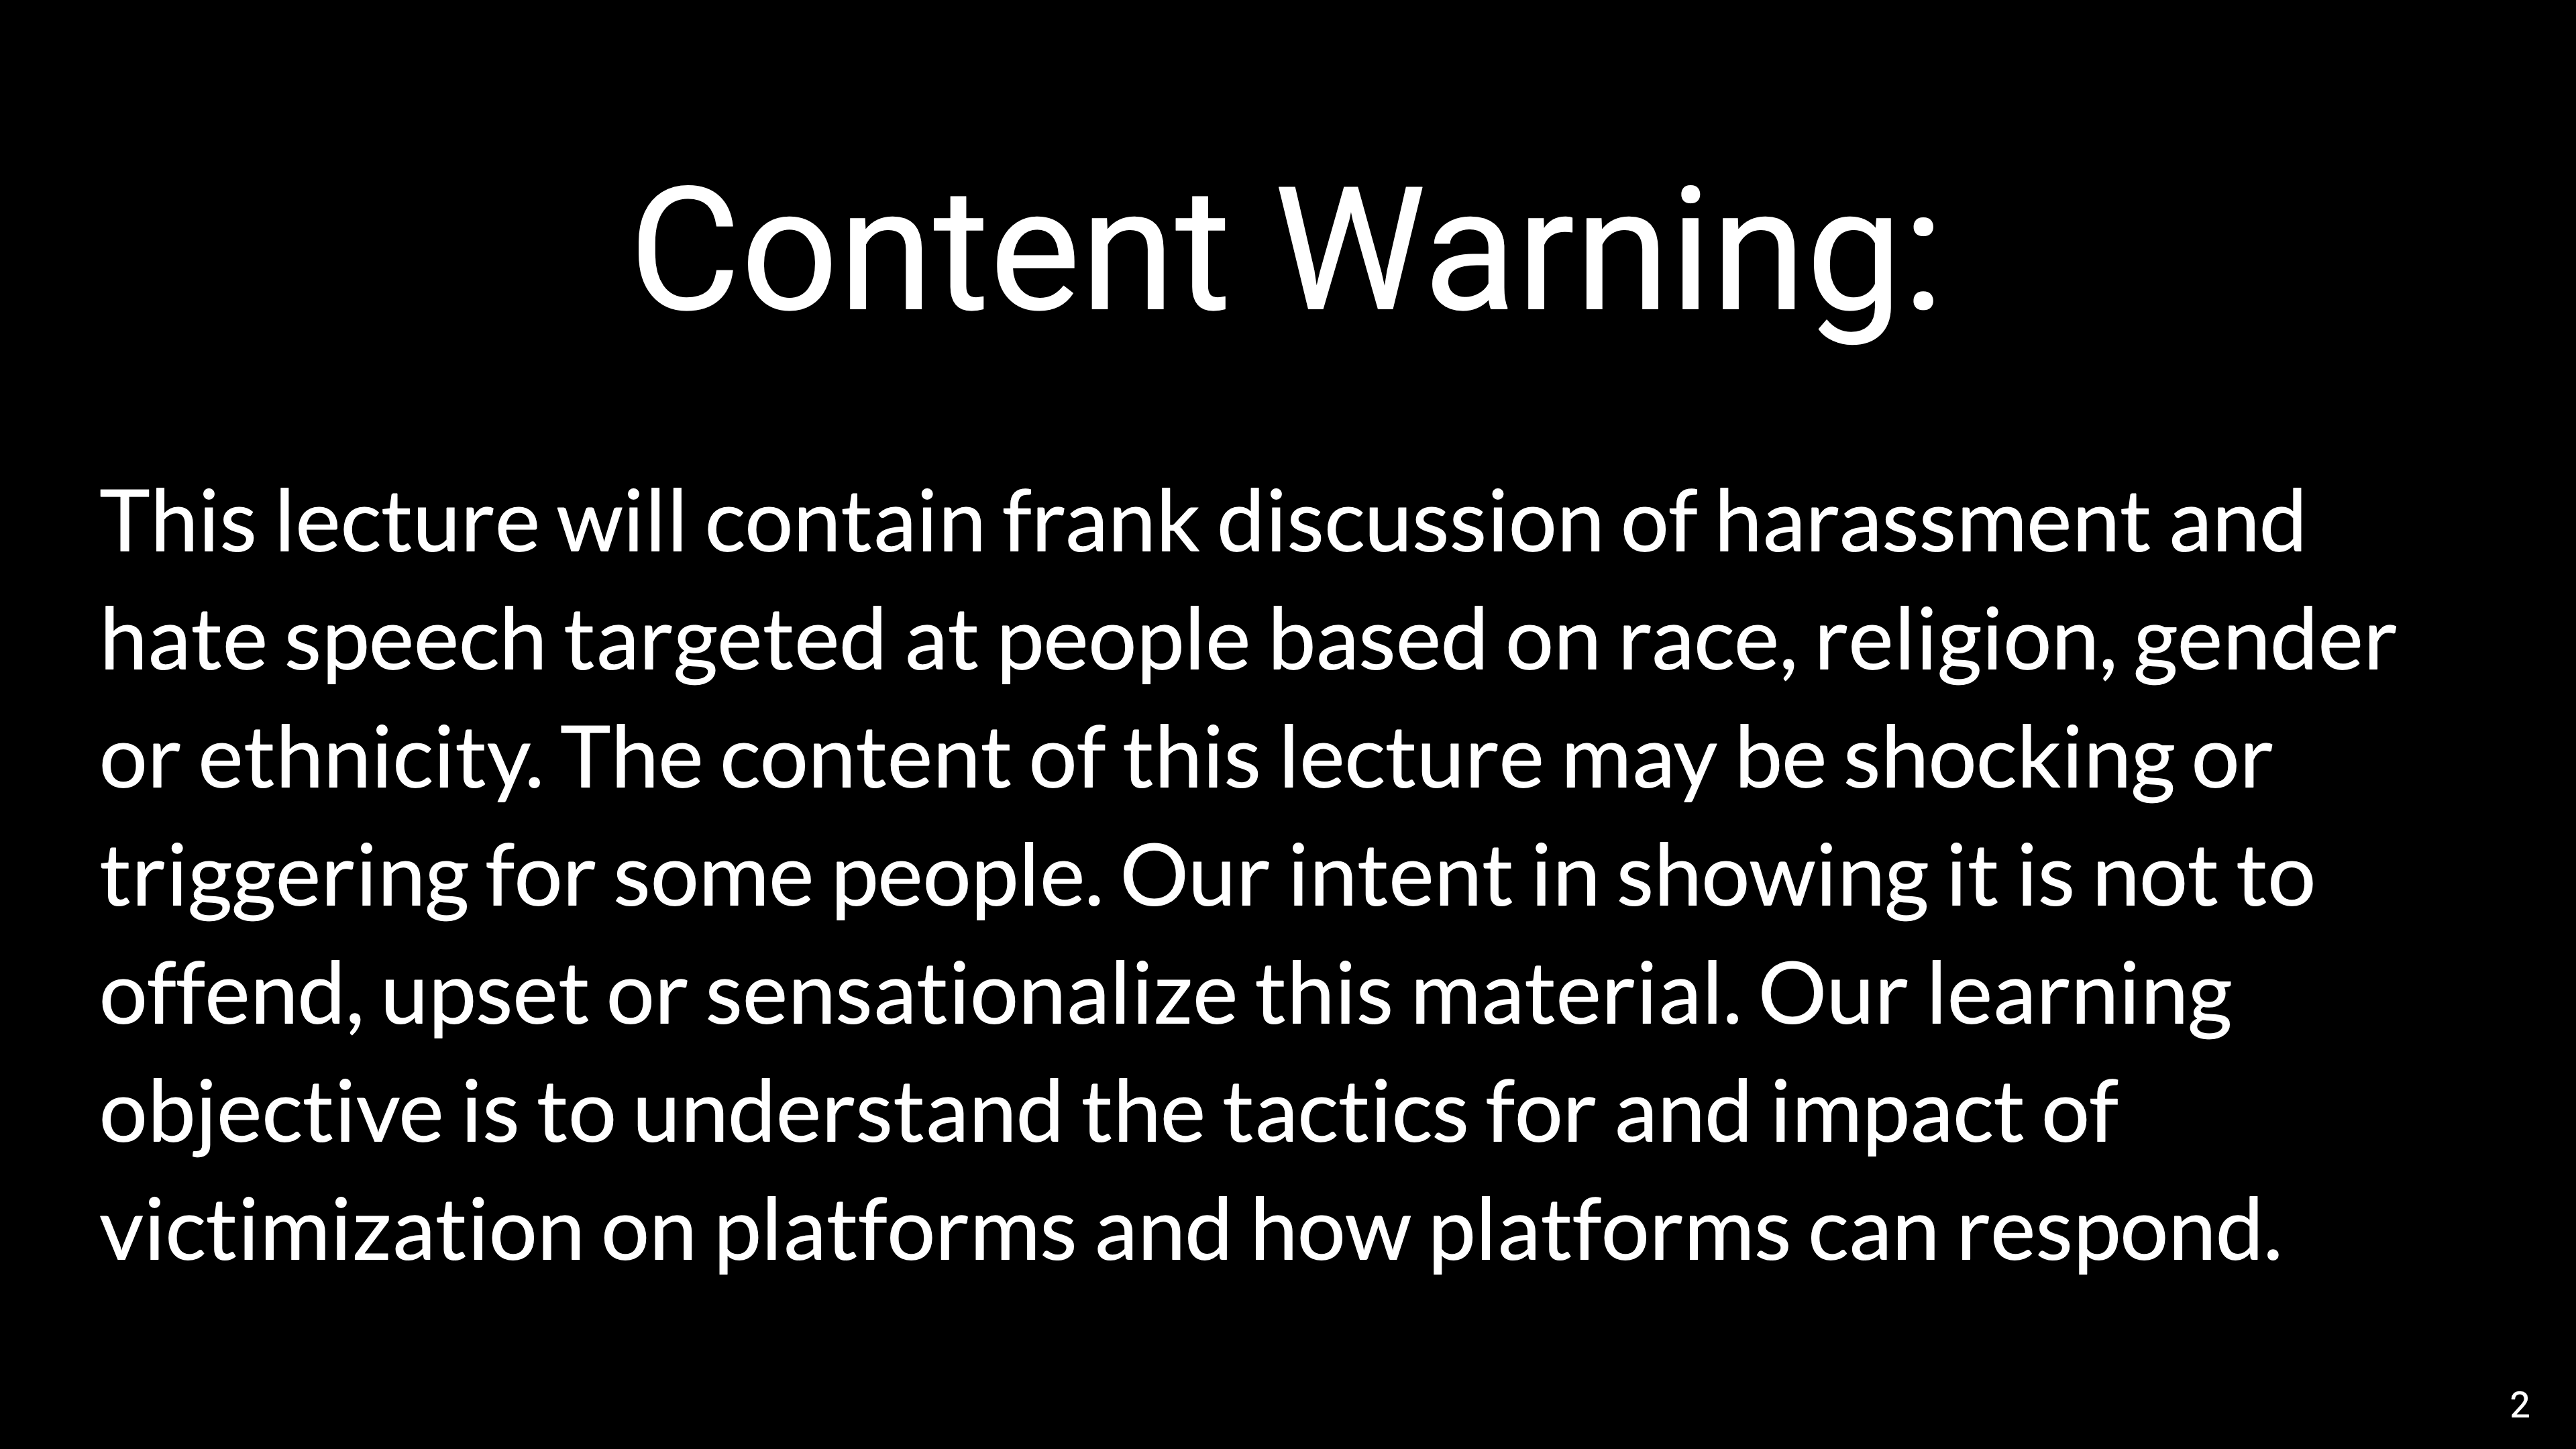
\includegraphics[width=\paperwidth]{content-warning}}
\end{frame}

\section{Victim Testimonial -- No recording, please}

\begin{frame}{What Will You Learn Today?}
    \large
    \begin{itemize}
        \item Harassment tactics: public and private
        \item Notable examples of harassment from the victim’s perspective
        \item Potential response strategies for various players
        \item Resources for targets of abuse
    \end{itemize}
\end{frame}

\section{Tactics}

\begin{frame}{Harassment Is Complicated and Adjacent to Many Other Abuses}
    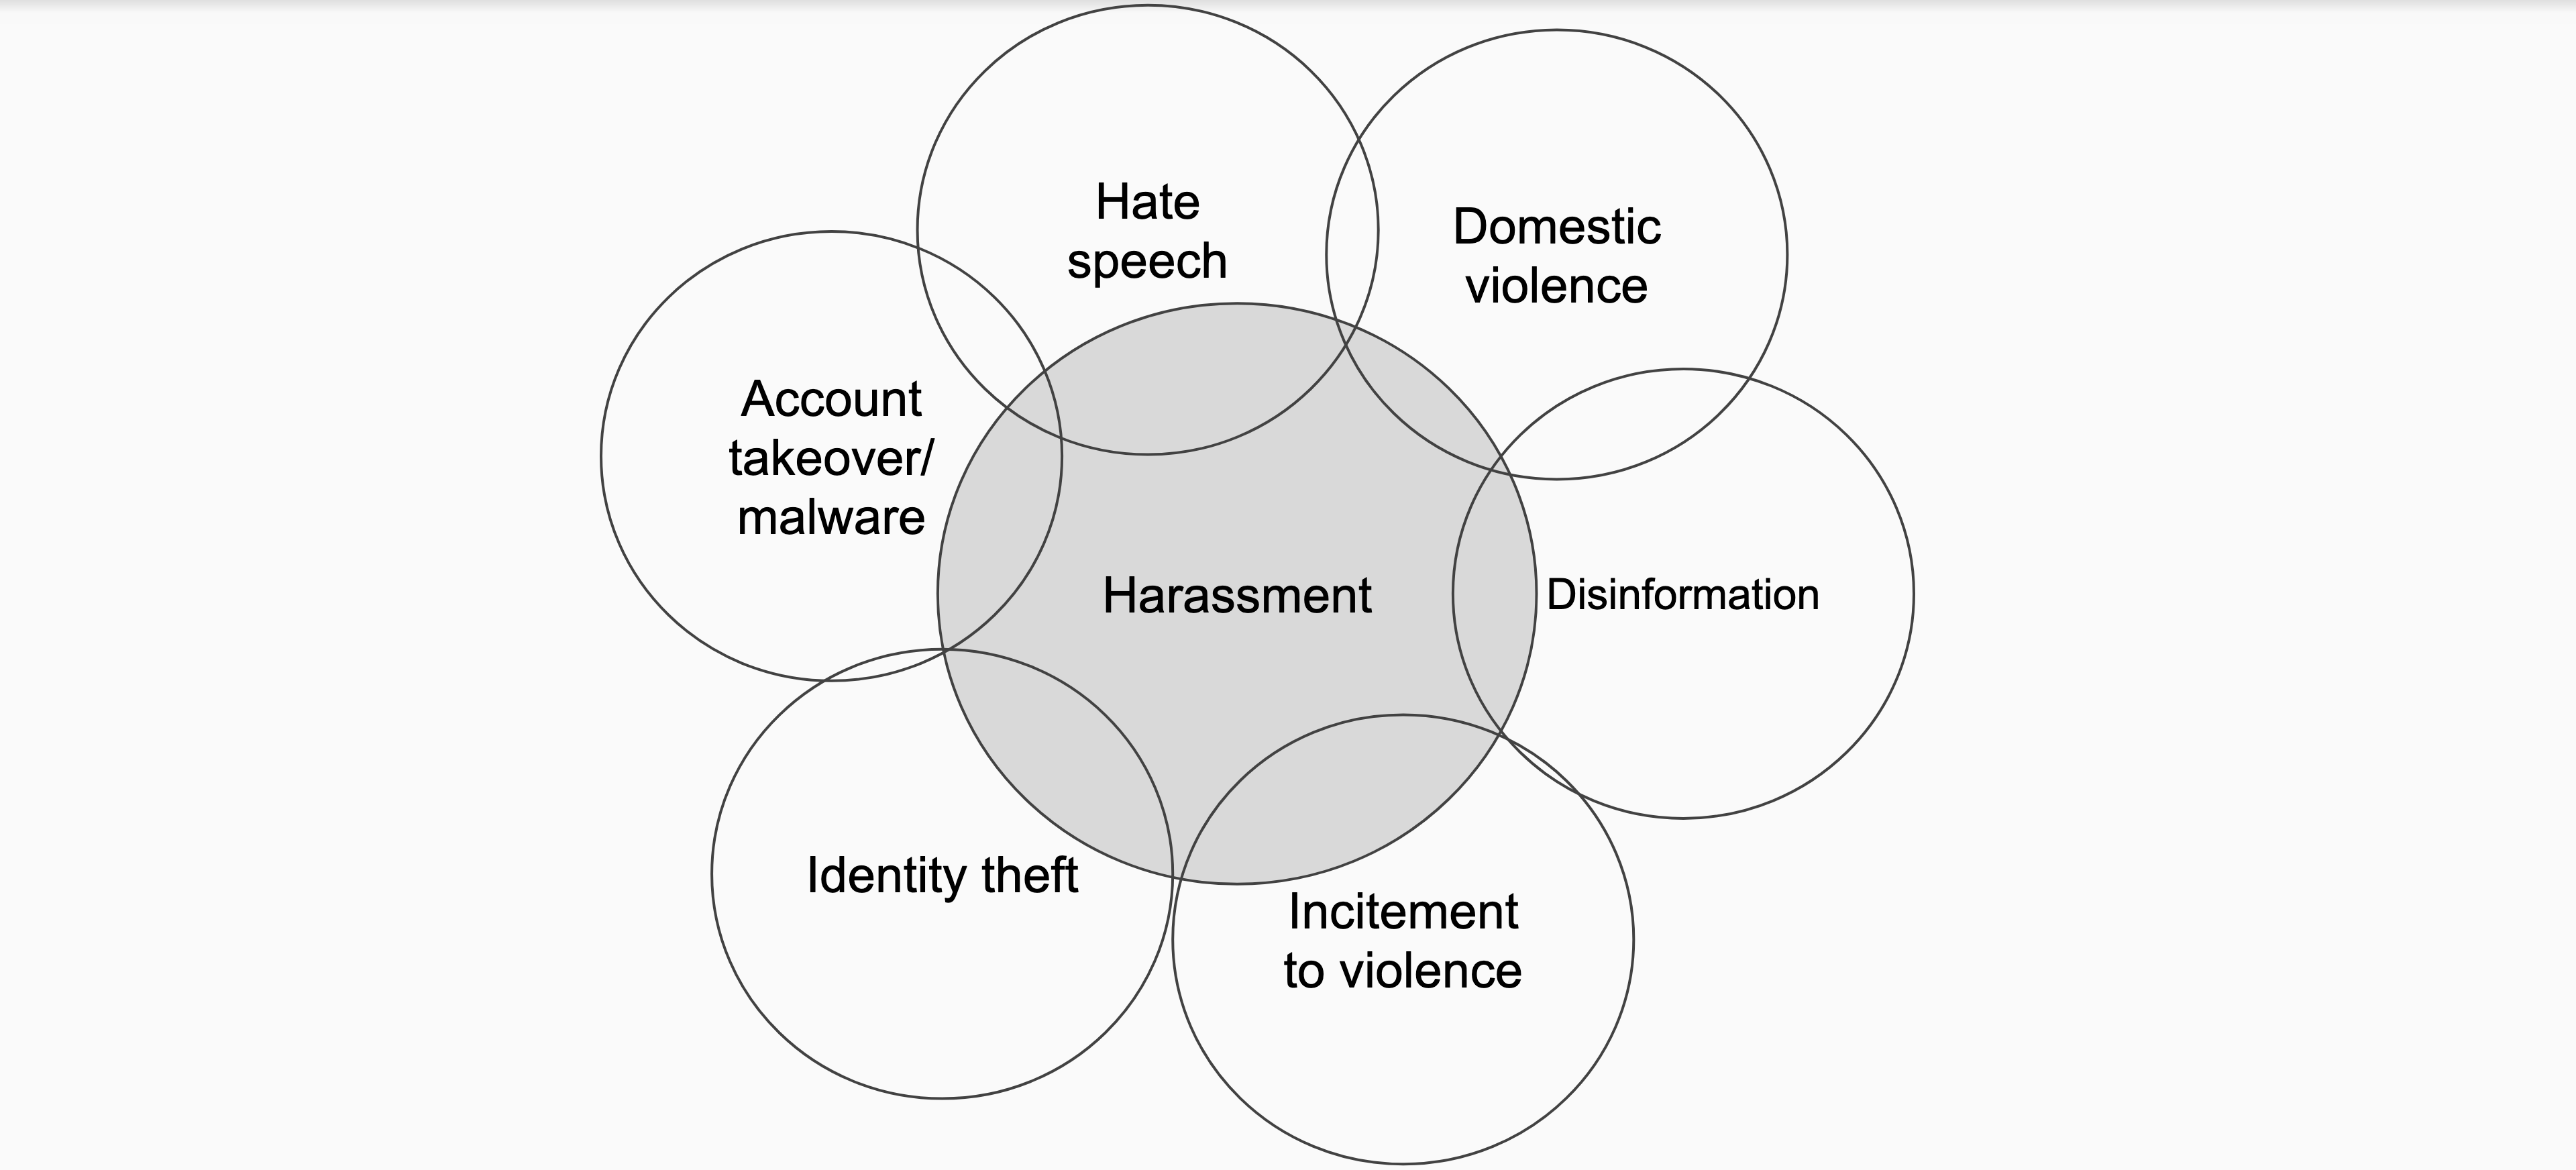
\includegraphics[width=\textwidth]{harassment-and-other-abuses}
\end{frame}

\begin{frame}{Trolling Tactics}
    \begin{columns}[T]
        \column{0.3\textwidth}
            \centering
            \large{\underline{\textbf{Public}}}\\~\\

            \small
            Swatting\\~\\
            Doxxing\\~\\
            Astroturfing\\~\\
            Extortion\\~\\
            Impersonation\\~\\
            Public Non-Consensual Intimate Imagery (NCII)\\~\\
            Sealioning
        \column{0.3\textwidth}
            \centering
            \large{\underline{\textbf{Communal}}}\\~\\

            \small
            Dogpiling\\~\\
            Group-to-individual harmful or threatening speech\\~\\
            Outreach to outside communities (school, church, employer, family)
        \column{0.3\textwidth}
            \centering
            \large{\underline{\textbf{Private}}}\\~\\

            \small
            Non-Consensual Intimate Imagery (NCII)\\~\\
            Individual-to-individual harmful or threatening speech\\~\\
            Email/text/platform based messaging\\~\\
            Cyberstalking\\~\\
            Catphishing\\~\\
            Sextortion
    \end{columns}
\end{frame}

\begin{frame}{Tactics Deep-Dive: Sealioning}
    \begin{columns}
        \column{0.3\textwidth}
            \footnotesize
            \begin{itemize}
                \item Users appear facially to be engaging in dialogue.
                \item However, the speaker intends to turn the tables on the target, inundating them with questions.
                \item When the target withdraws, the speaker claims that they were the one who was attempting to be open and civil.
            \end{itemize}
        \column{0.75\textwidth}
            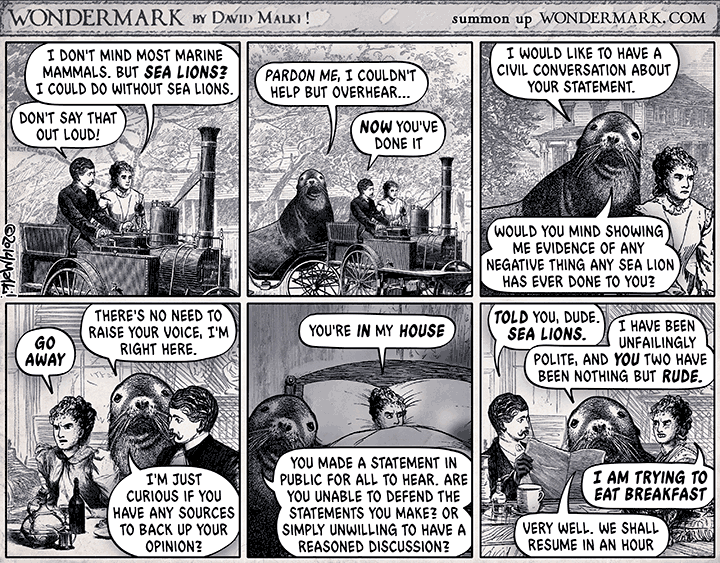
\includegraphics[width=\textwidth]{sealioning-comic}
    \end{columns}
\end{frame}

\begin{frame}{Tactics Deep-Dive: Dogpiling}
    \begin{columns}[T]
        \column{0.4\textwidth}
            \scriptsize
            \begin{itemize}
                \item Reliant on cybermobs.
                \item Often targeted based on personal characteristics (e.g. race, ethnicity, religion, gender, sexual orientation, sexual identity) or by expressing unpopular opinions.
                \item Target is then overwhelmed with negative content by an online mob.
                \item Goal is to make the person so tired of dealing with abuse that they either recant, withdraw, or are driven from online spaces completely.
                \item Sometimes the dogpiling is so extreme that a person can no longer participate in online forums.
            \end{itemize}
        \column{0.6\textwidth}
            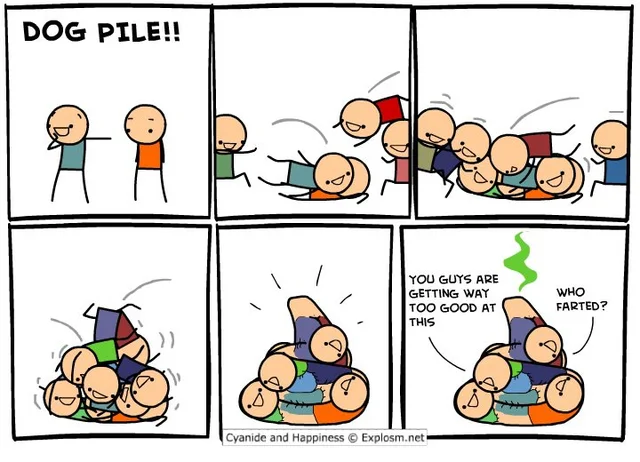
\includegraphics[width=\textwidth]{dogpile-cyanide-and-happiness}
    \end{columns}
\end{frame}

\begin{frame}{Tactics Deep-Dive: Swatting}
    \begin{columns}
        \column{0.5\textwidth}
            \scriptsize
            \begin{itemize}
                \item Hoax call placed to law enforcement detailing a completely false but plausibly life-threatening event that the caller claims is taking place in a target’s home or business. E.g. false reporting of a serious law enforcement emergency, such as a bomb threat, shooting, murder, hostage situation.
                \item Police and emergency response teams show up to a target’s home fully armed, putting the target and their family in grave danger.
                \item Swattings are common within gamer communities and often target celebrities and public figures.
                \item Uninvolved man shot \& killed as a result of his address being used in a gaming dispute \& swatting in December 2017.
            \end{itemize}
        \column{0.5\textwidth}
            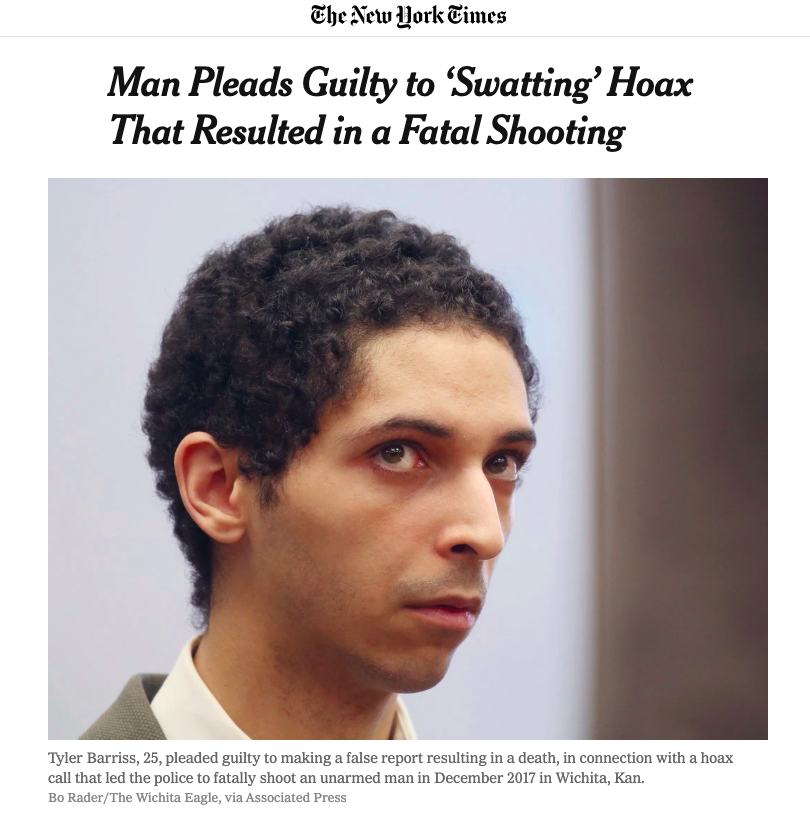
\includegraphics[width=\textwidth]{swatting-nyt}
    \end{columns}
\end{frame}

\section{Examples of Harassment}

\begin{frame}{Foundational Harassment Case: Gamergate}
    \begin{columns}
        \column{0.4\textwidth}
            \begin{itemize}
                \item Triggered by real-life boyfriend but picked up by strangers
                \item Coordinated dogpiling through many attack channels against a small number of female game designers
                \item Included doxxing, account hacking, revenge porn, and creation of vast amount of disinformation to confuse neutral observers
                \item Possibly amplified by foreign disinformation actors
            \end{itemize}
        \column{0.6\textwidth}
            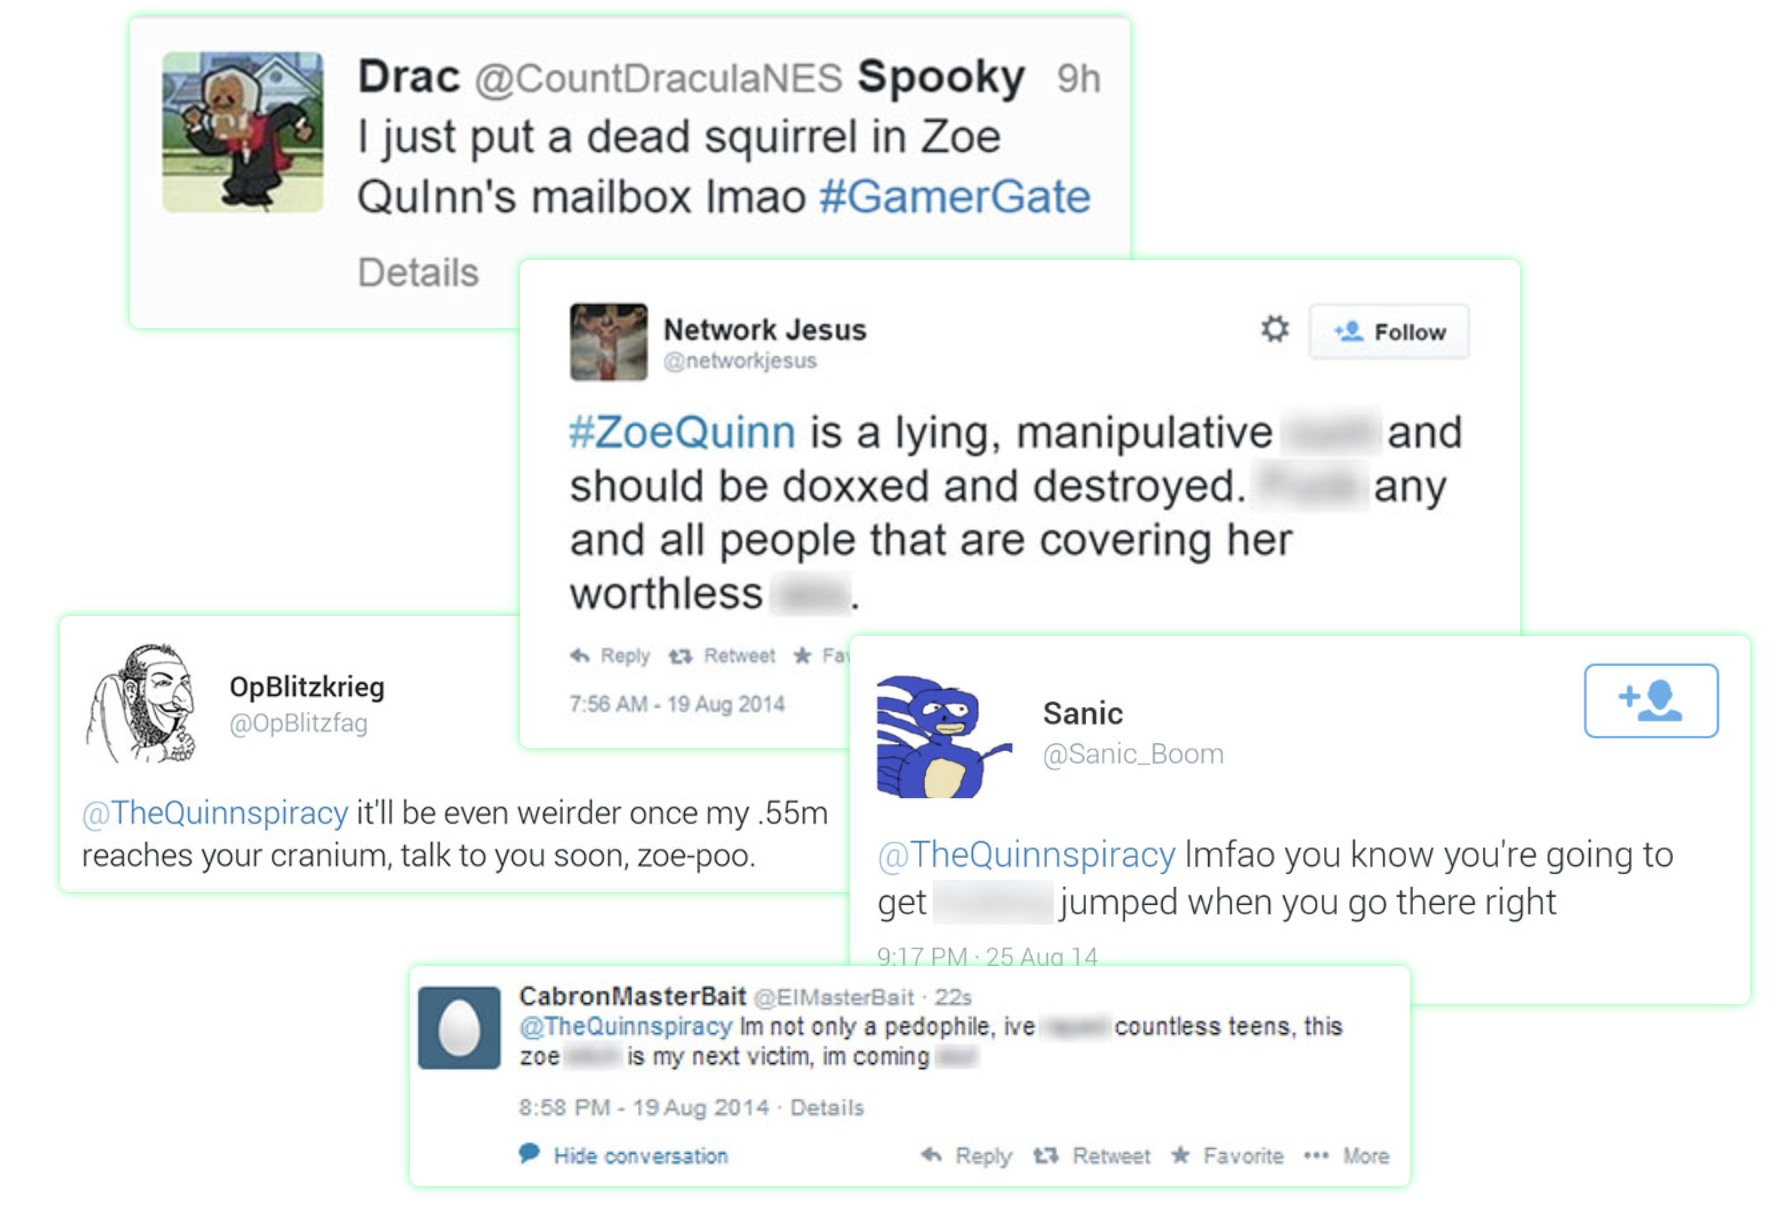
\includegraphics[width=\textwidth]{zoe-quinn-harassment-tweets}
            \begin{columns}
                \column{0.4\textwidth}
                    
\includegraphics[width=\textwidth]{zoe-quinn}
                \column{0.6\textwidth}
                    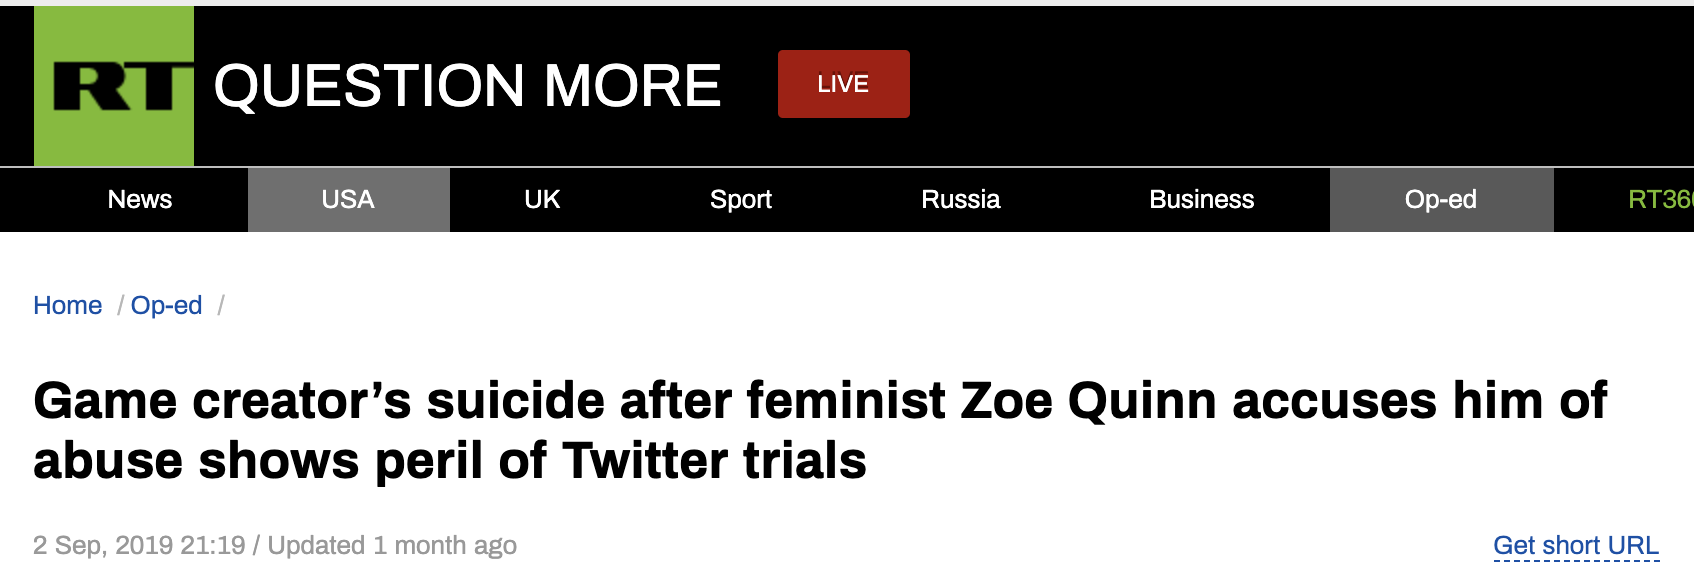
\includegraphics[width=\textwidth]{rt-zoe-quinn}
            \end{columns}
    \end{columns}
\end{frame}

\begin{frame}{Impersonation}
    \begin{columns}
        \column{0.5\textwidth}
            \centering
            \small
            Impersonation of a potential romantic partner is known as “catfishing” -- but assuming another’s identity online can result in havoc in their professional and personal lives.
            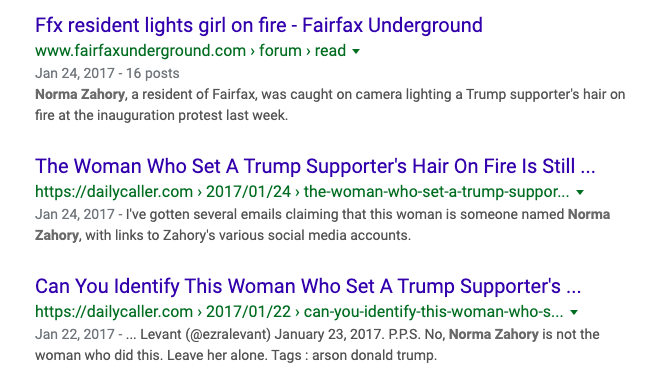
\includegraphics[width=\textwidth]{hair-on-fire-search}
        \column{0.5\textwidth}
            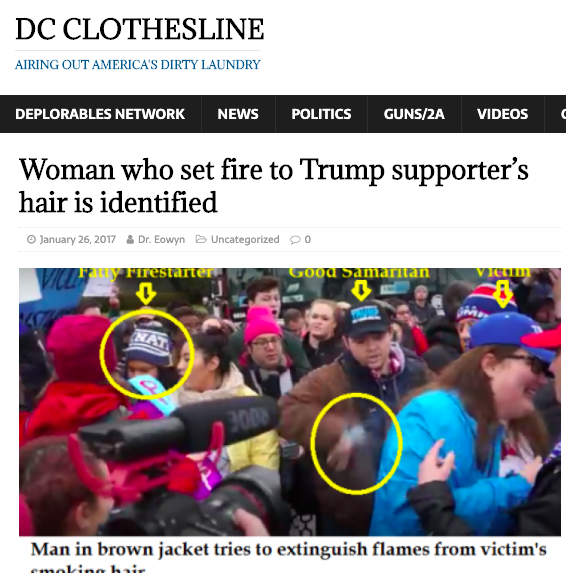
\includegraphics[width=\textwidth]{hair-on-fire-article}
    \end{columns}
\end{frame}

\begin{frame}{Targeting Journalists to Silence Voices}
    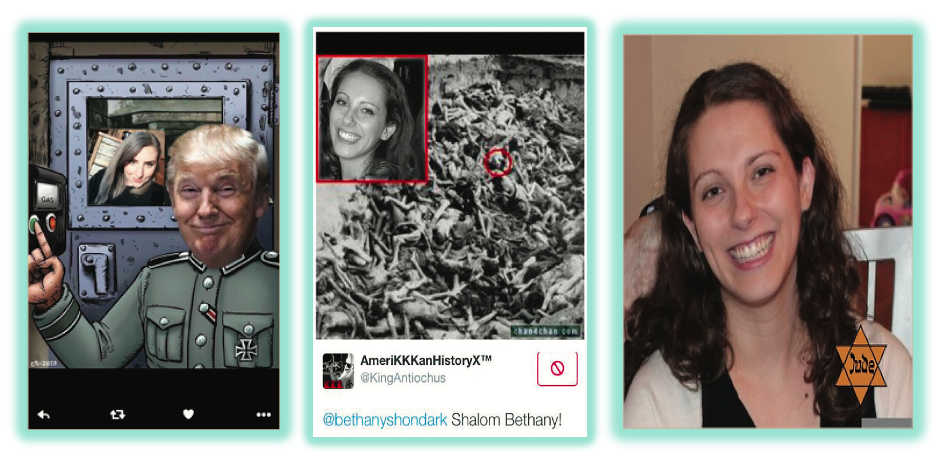
\includegraphics[width=\textwidth]{targeting-journalists}
\end{frame}

\begin{frame}{Targeting Journalists to Silence Voices}
    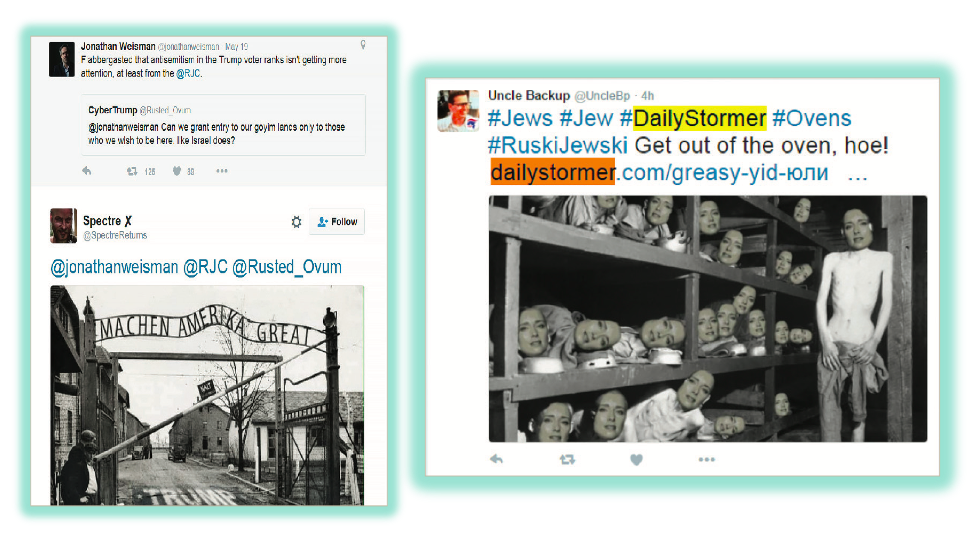
\includegraphics[width=0.65\textwidth]{silencing-journalists-holocaust}
    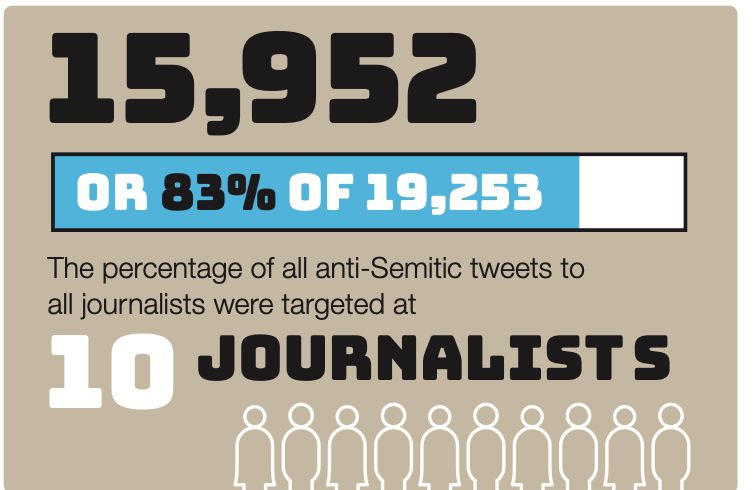
\includegraphics[width=0.3\textwidth]{anti-semitic-tweets-stats}
\end{frame}

\begin{frame}{Taylor Dumpson}
    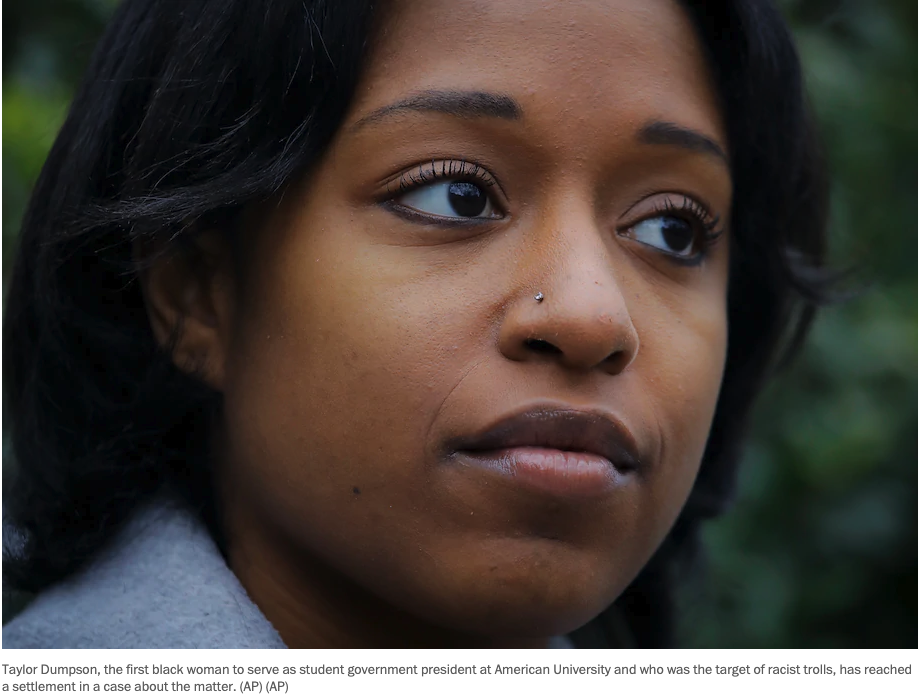
\includegraphics[width=\textwidth]{taylor-dumpson}
\end{frame}

\begin{frame}{Doxxing Dissidents: Russia}
    
\includegraphics[width=\textwidth]{russian-dissident}
\end{frame}

\begin{frame}{Targeting the Moderators}
    
\includegraphics[width=\textwidth]{conway-roth}
    
\includegraphics[width=0.6\textwidth]{conway-roth-headline}
\end{frame}

\begin{frame}{A Combination of Numerous Tactics: Amanda Todd}
    \begin{columns}
        \column{0.4\textwidth}
            
\includegraphics[width=\textwidth]{i-have-nobody}
        \column{0.6\textwidth}
            \begin{itemize}
                \item Case combined cyberstalking, sextortion, doxxing, child sexual abuse, and real life harassment.
                \item What happens online has real life consequences.
            \end{itemize}
            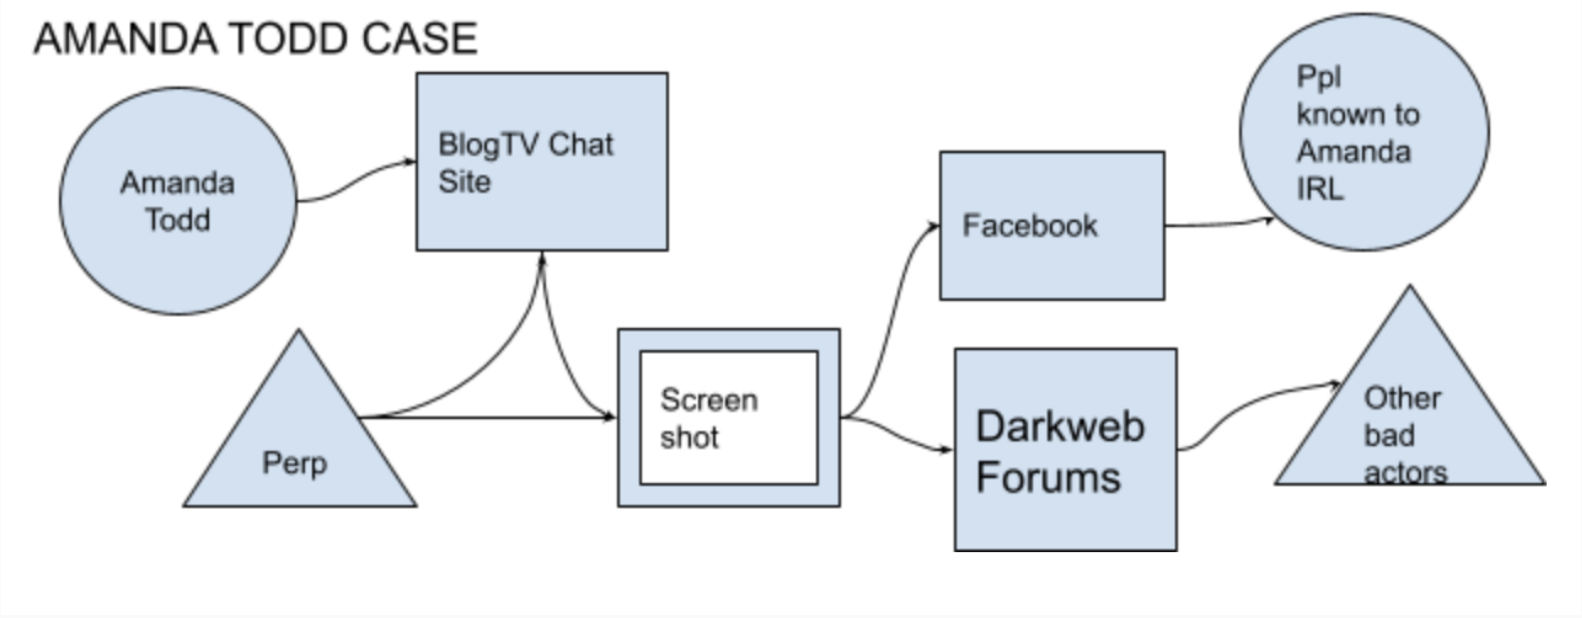
\includegraphics[width=\textwidth]{amanda-todd-case}
    \end{columns}
\end{frame}

\section{Responses and Mitigations}

\begin{frame}{Policy Responses}
    \begin{enumerate}
        \item Set clear policies 
        \item Partnerships: know the players
        \item Protection of public figures - especially young ones
        \item Partnerships and Education
    \end{enumerate}
\end{frame}

\begin{frame}{Set Clear Policies for Awful but Lawful Content}
    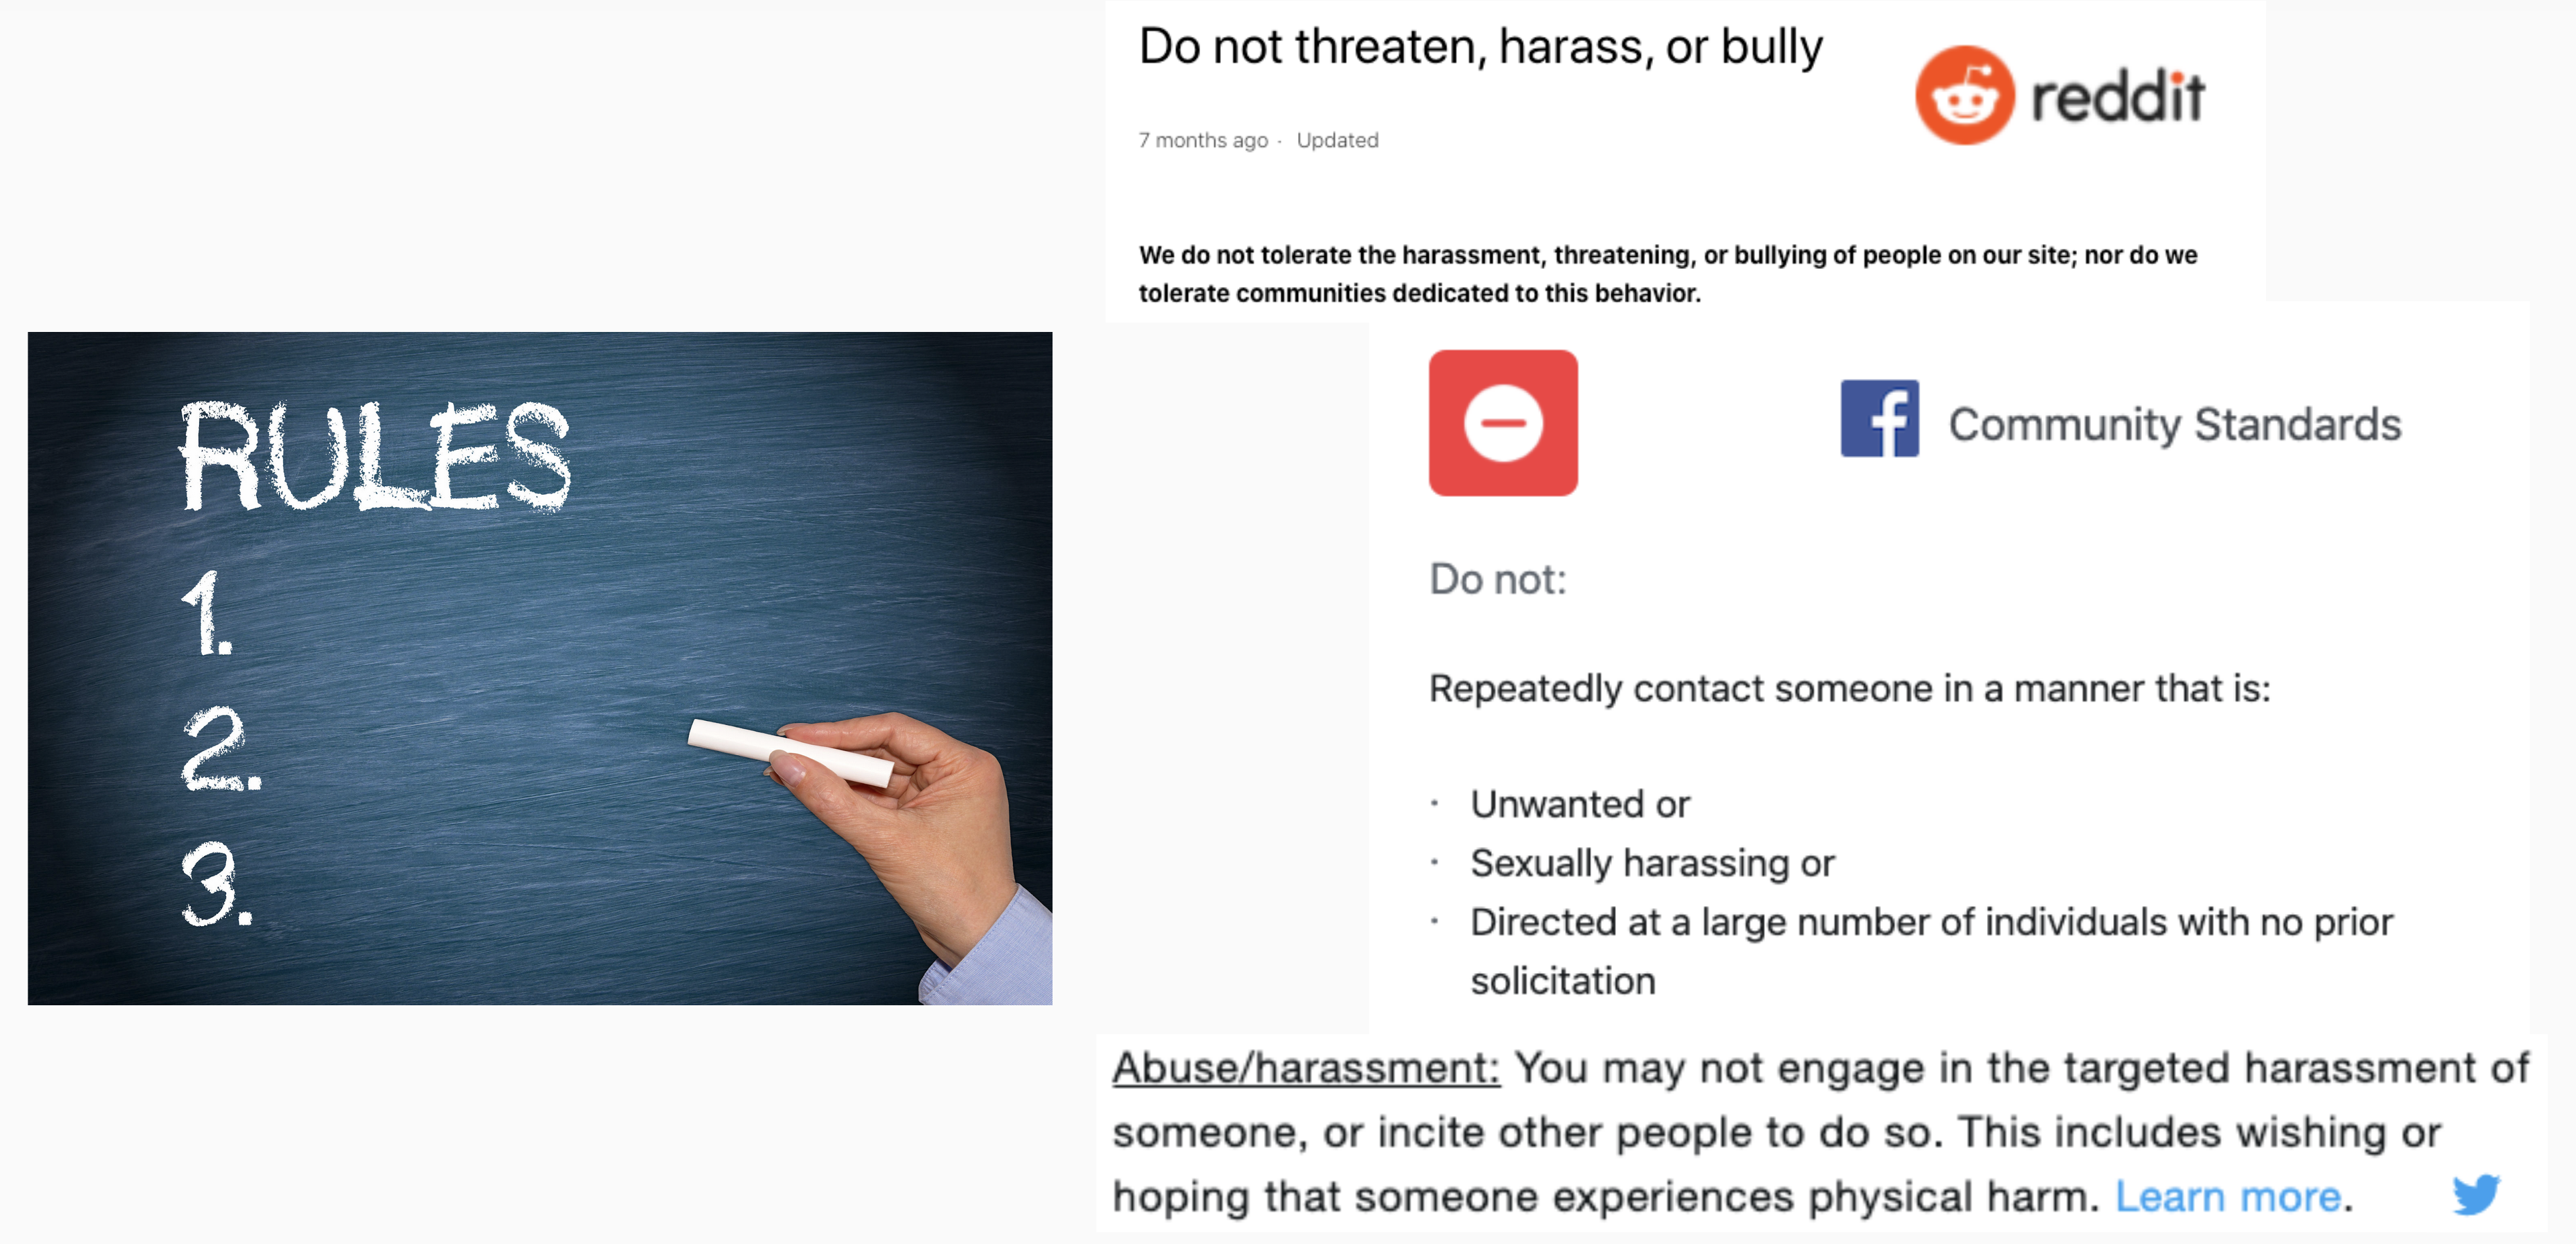
\includegraphics[width=\textwidth]{content-policies}
\end{frame}

\begin{frame}{Dogpiling or Accountability?}
    \begin{columns}[T]
        \column{0.25\textwidth}
            
\includegraphics[trim=0 0 0 0, clip, height=0.3\textheight]{justine-sacco}
            \textbf{Justine Sacco}\\~\\
            Tweets racist joke to 170 followers, gets on plane, fired by landing
        \column{0.25\textwidth}
            
\includegraphics[height=0.3\textheight]{emmanuel-cafferty}
            \textbf{Emmanuel Cafferty}\\~\\
            SDG\&E lineman, stranger posts photo to Twitter of his fingers in an “OK” sign, is doxxed and fired
        \column{0.25\textwidth}
            
\includegraphics[trim=220 0 140 0, clip, height=0.3\textheight]{amy-cooper}
            \textbf{Amy Cooper}\\~\\
            Calls cops on innocent black birdwatcher. Fired, doxxed, lost dog, charged by NY DA, plead out
        \column{0.25\textwidth}
            \includegraphics[trim=200 800 250 200, clip, height=0.3\textheight]{sarah-jeong}
            \textbf{Sarah Jeong}\\~\\
            Tech journalist, gets job at NYT. Old tweets unearthed, massive abuse thrown her way
    \end{columns}
\end{frame}

\begin{frame}{Potential Partners}
    \begin{enumerate}
        \item Targets
        \item Victim advocates
        \item Organizations vulnerable to manipulation
        \item Law enforcement
        \item Lawmakers
        \item Platforms
    \end{enumerate}
\end{frame}

\begin{frame}{Targets}
    \begin{columns}
        \column{0.5\textwidth}
            \begin{itemize}
                \item Harassment is pervasive!
                \item Targets report being “not listened to” when they go to platforms.
                \item Many technical solutions place the onus on \textbf{targets themselves} to proactively report harassment and bullying.
                \item Whack-a-mole for victims, especially with cross-platform harassment 
            \end{itemize}
        \column{0.5\textwidth}
            \centering
            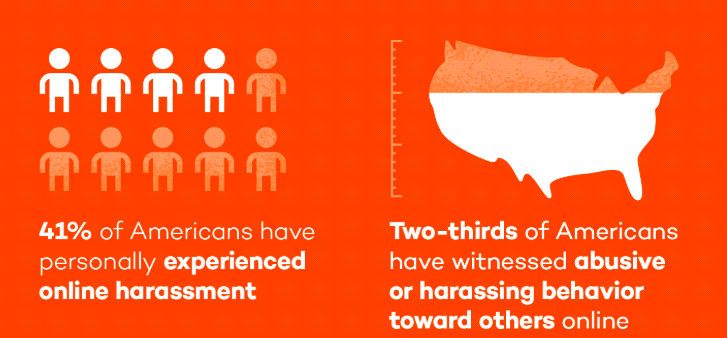
\includegraphics[width=\textwidth]{harassment-stats}
            
\includegraphics[width=\textwidth]{whack-a-mole-kitten}
    \end{columns}
\end{frame}

\begin{frame}{Victim Advocates}
    
\includegraphics[width=\textwidth]{victim-advocates}
\end{frame}

\begin{frame}{Law Enforcement \& Bullying Laws Across America}
    \begin{columns}
        \column{0.4\textwidth}
            
\includegraphics[width=\textwidth]{cyberbullying-research-center}
            \begin{itemize}
                \item LE often first POC
                \item Non-sophisticated departments will often tell targets to “turn off their screens” or will not have the sophistication/resources to investigate cyberharassment.
            \end{itemize}
        \column{0.6\textwidth}
            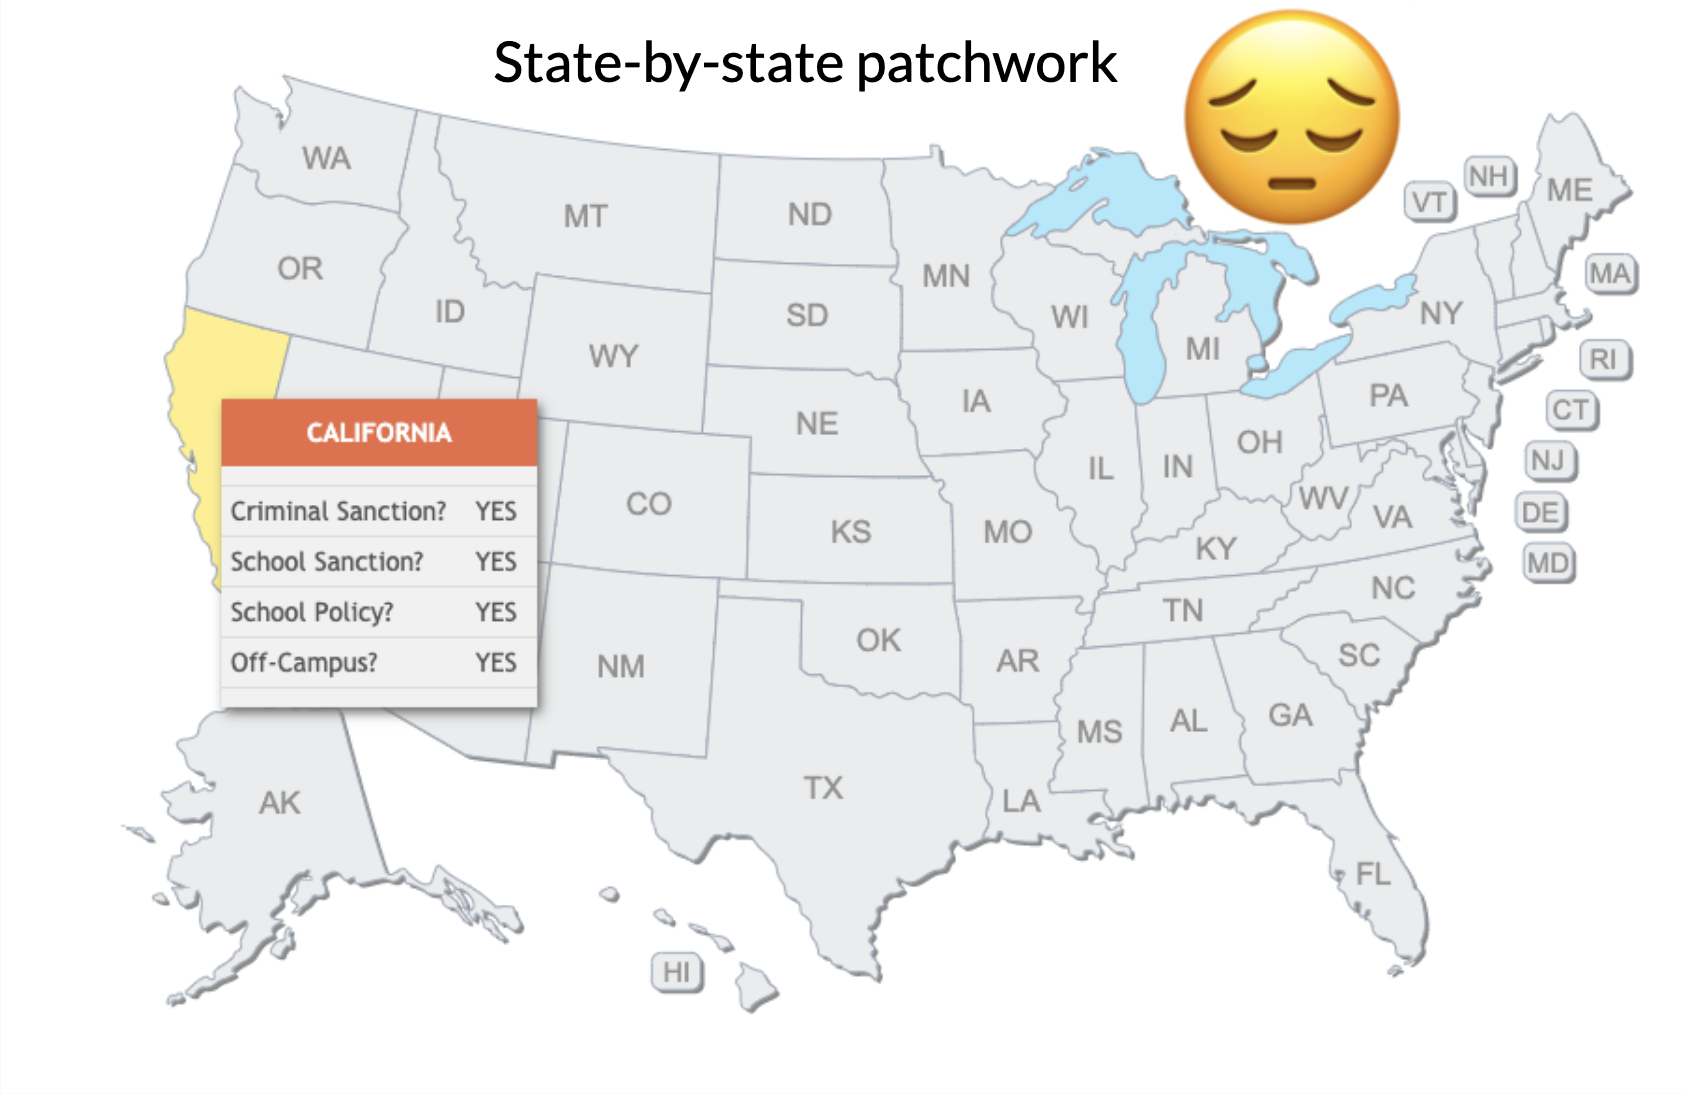
\includegraphics[width=\textwidth]{bullying-laws-map}
    \end{columns}
\end{frame}

\begin{frame}{}
    Despite the gravity of their predicaments, cyberharassment victims are often told that nothing can or should be done about online abuse. . . . If victims seek legal help, they are accused of endangering the internet as a forum of public discourse. . . . These views are wrongheaded and counterproductive.\\
    – Danielle Keats Citron, \textit{Hate Crimes in Cyberspace}
\end{frame}

\begin{frame}{Product/Technical Responses}
    \begin{enumerate}
        \item Reporting flows
        \item Proactive monitoring and measurement
        \item Productive friction
        \item User-controls
        \item Shadow-blocking
        \item Third-party tools
    \end{enumerate}
\end{frame}

\begin{frame}{Example Reporting Flows: WhatsApp}
    \centering
    
\includegraphics[width=25pt]{whatsapp}
    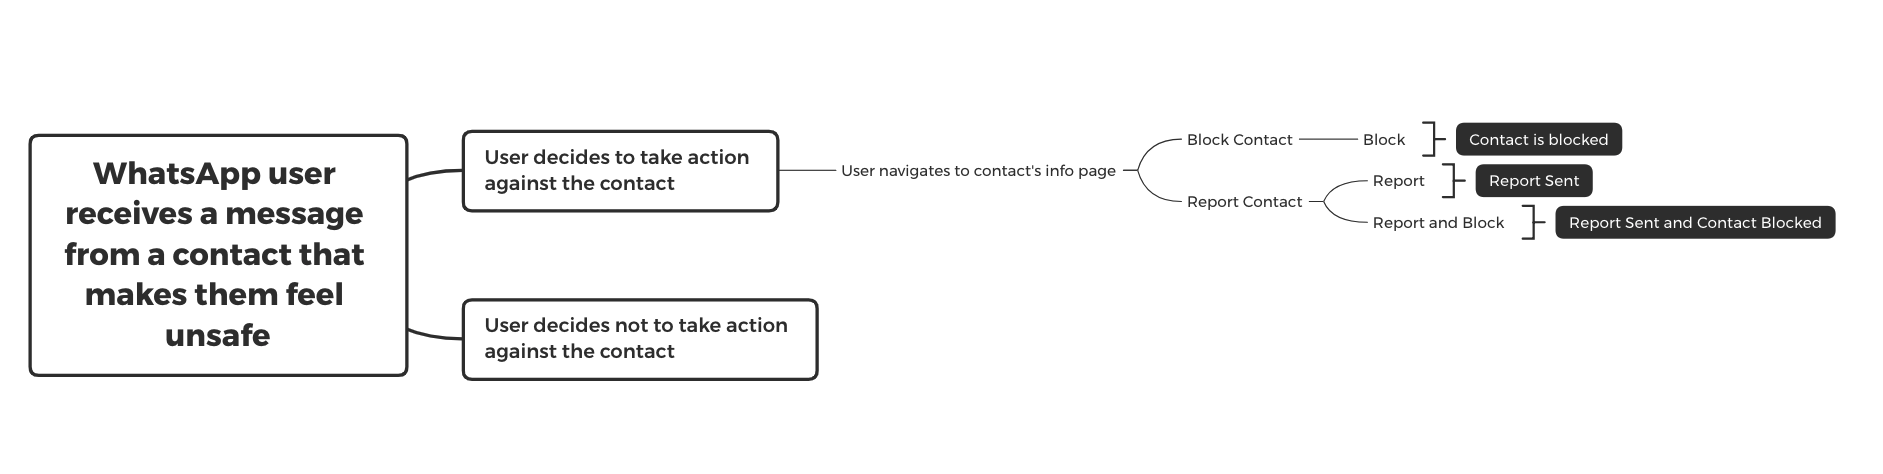
\includegraphics[width=\textwidth]{whatsapp-reporting-flow}
\end{frame}

\begin{frame}{Example Reporting Flows: Facebook}
    \centering
    
\includegraphics[width=25pt]{facebook}
    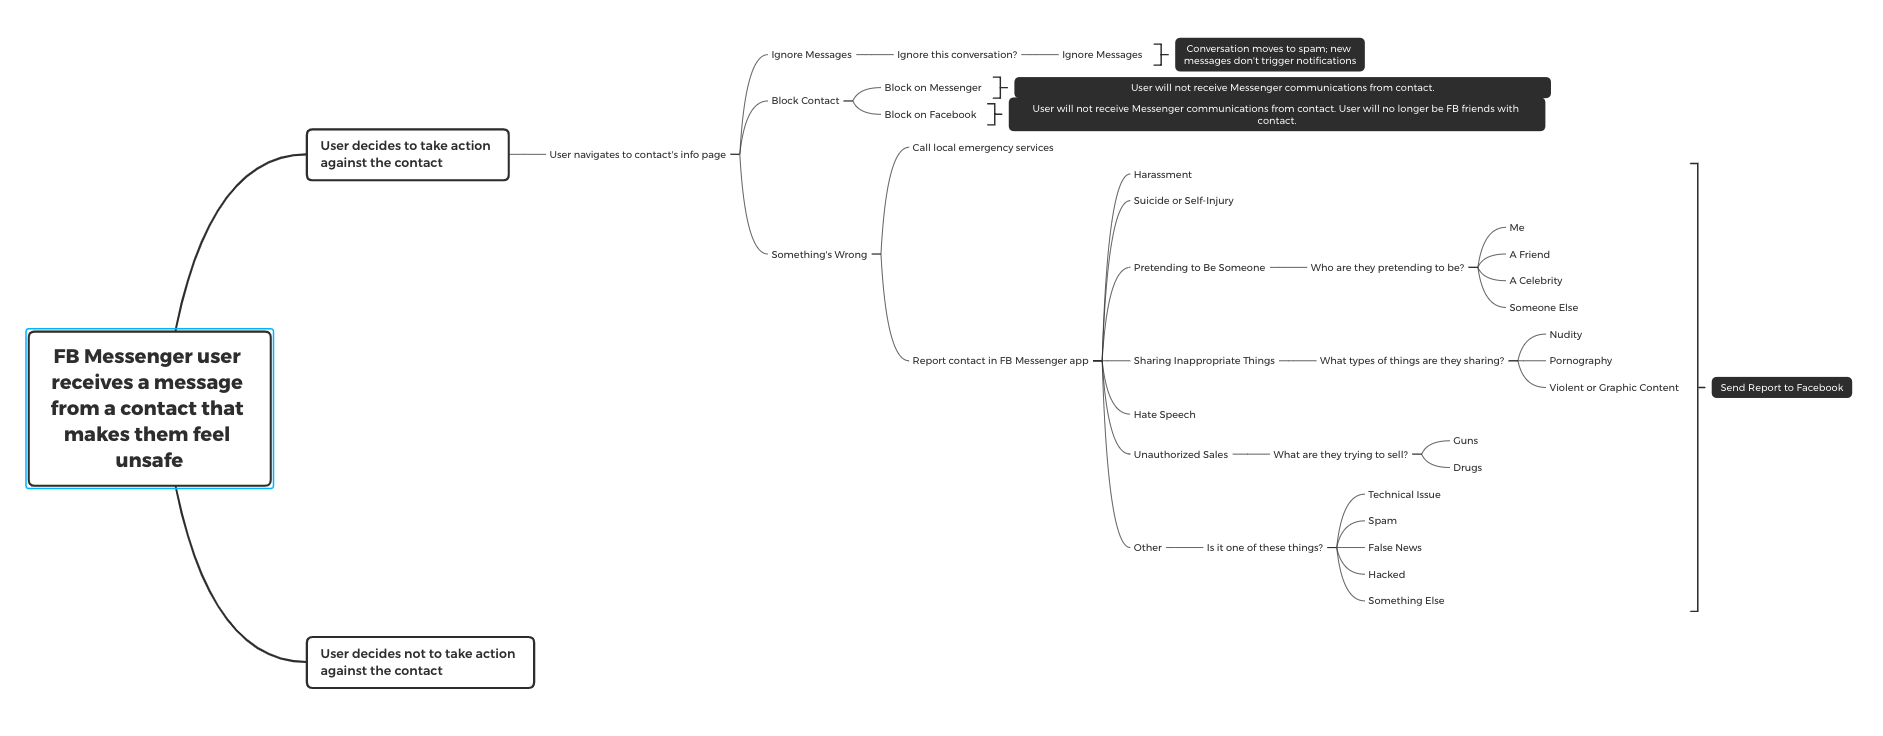
\includegraphics[width=\textwidth]{facebook-reporting-flow}
\end{frame}

\begin{frame}{Example Reporting Flows: Reddit}
    \centering
    
\includegraphics[width=25pt]{reddit}
    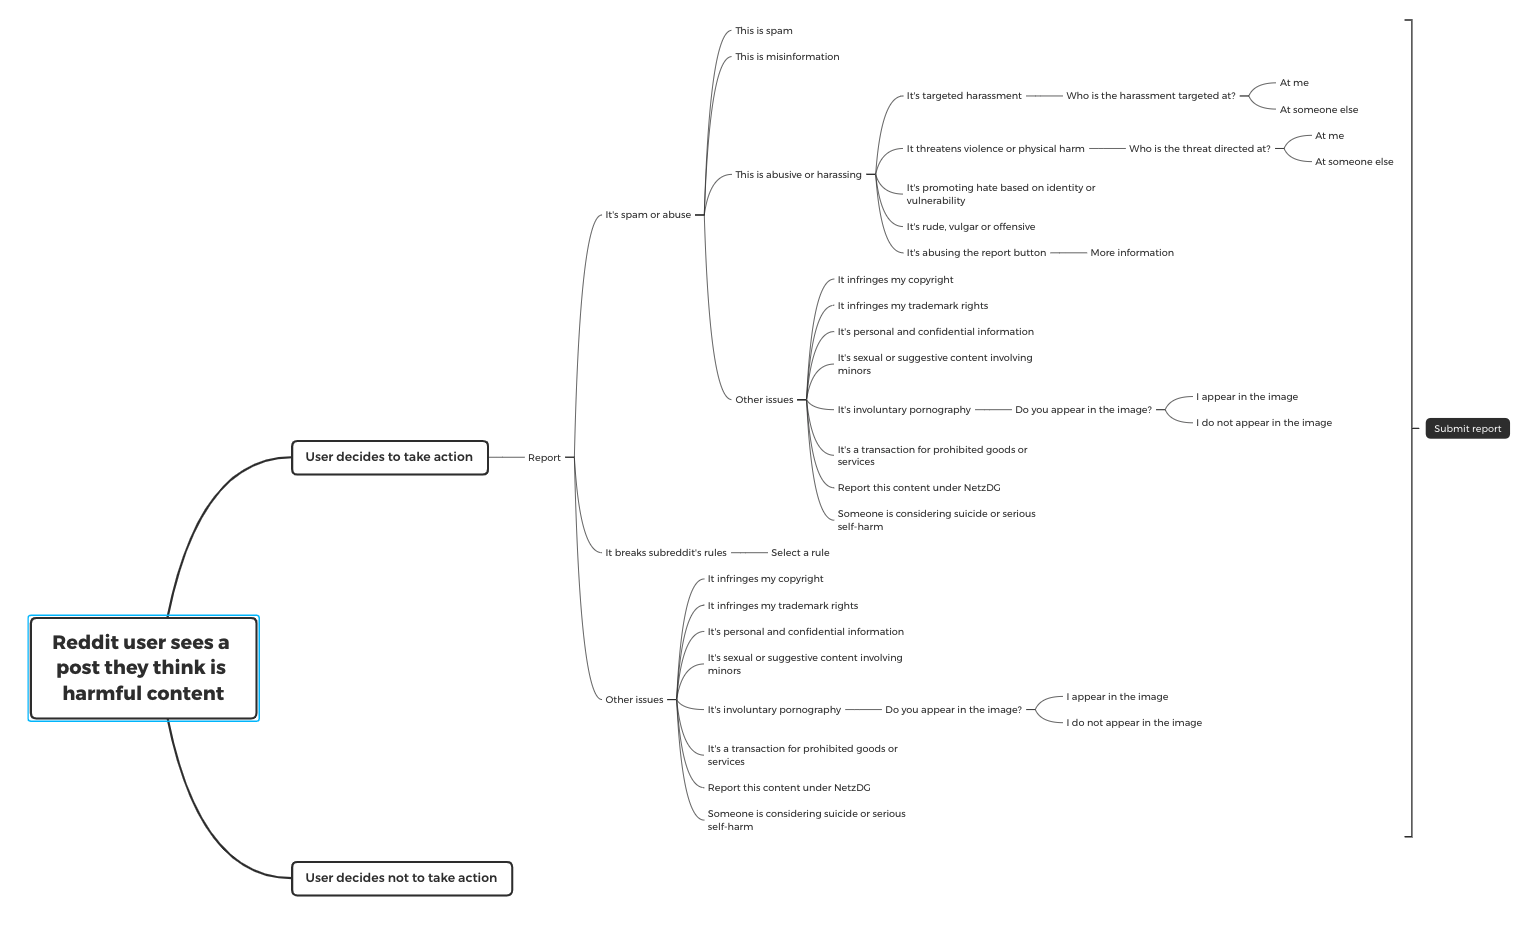
\includegraphics[width=\textwidth]{reddit-reporting-flow}
\end{frame}

\begin{frame}{Example Reporting Flows: Telegram}
    \centering
    
\includegraphics[width=70pt]{telegram}
    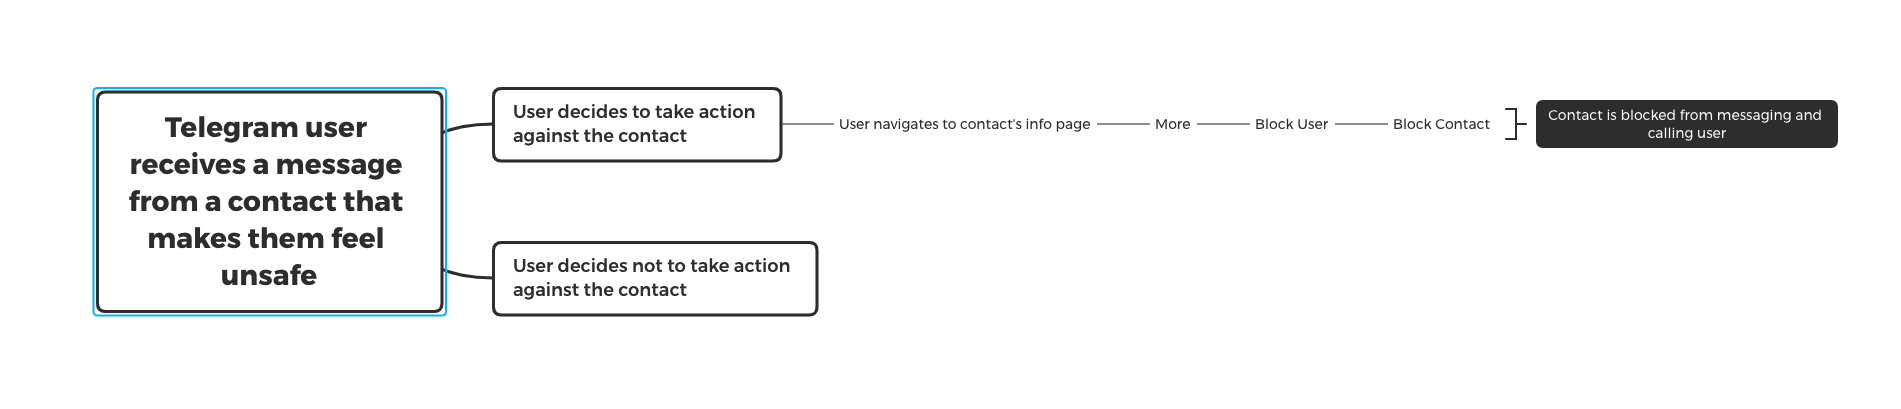
\includegraphics[width=\textwidth]{telegram-reporting-flow}
\end{frame}

\begin{frame}{Go to your favorite app and (almost) report your friend!}
    
\includegraphics[width=0.5\textwidth]{block-alex-stamos-1}
    
\includegraphics[width=0.3\textwidth]{block-alex-stamos-2}
\end{frame}

\begin{frame}{Characteristics of a Good Reporting Flow}
    \begin{itemize}
        \item Terms of service (TOS) are \underline{clear and consistently applied}
        \item \underline{Encourage users to take action} (eg. block other user from viewing profile/muting a user)
        \item \underline{Easy to complete} with clear choices or categories for a user to choose from when asked to classify report
        \item Gives \underline{adequate data for queuing and ranking}
        \item Differ in \underline{private and public} spaces
    \end{itemize}
\end{frame}

\begin{frame}{Public Reporting}
    \begin{itemize}
        \item Automated flagging and reporting of messages that meet a harmfulness threshold
        \begin{itemize}
            \item Messages may be immediately removed or flagged for moderator review
        \end{itemize}
        \item User reports of messages
    \end{itemize}
    
\includegraphics[width=\textwidth]{show-offensive-content-twitter}
\end{frame}

\begin{frame}{Private Reporting}
    \begin{columns}
        \column{0.55\textwidth}
            \begin{itemize}
                \item In order to report harmful content, users must at least: 
                \begin{itemize}
                    \item Have awareness on the how and why of reporting
                    \item Believe that reports are being processed in a meaningful way that promotes their safety while maintaining privacy
                \end{itemize}
                \item Reporting can be tied to: 
                \begin{itemize}
                    \item Accounts
                    \item Conversations
                    \item Messages
                \end{itemize}
                \item Specificity => effectiveness of operational teams
            \end{itemize}
        \column{0.45\textwidth}
            
\includegraphics[width=0.49\textwidth]{block-alex-stamos-2}
            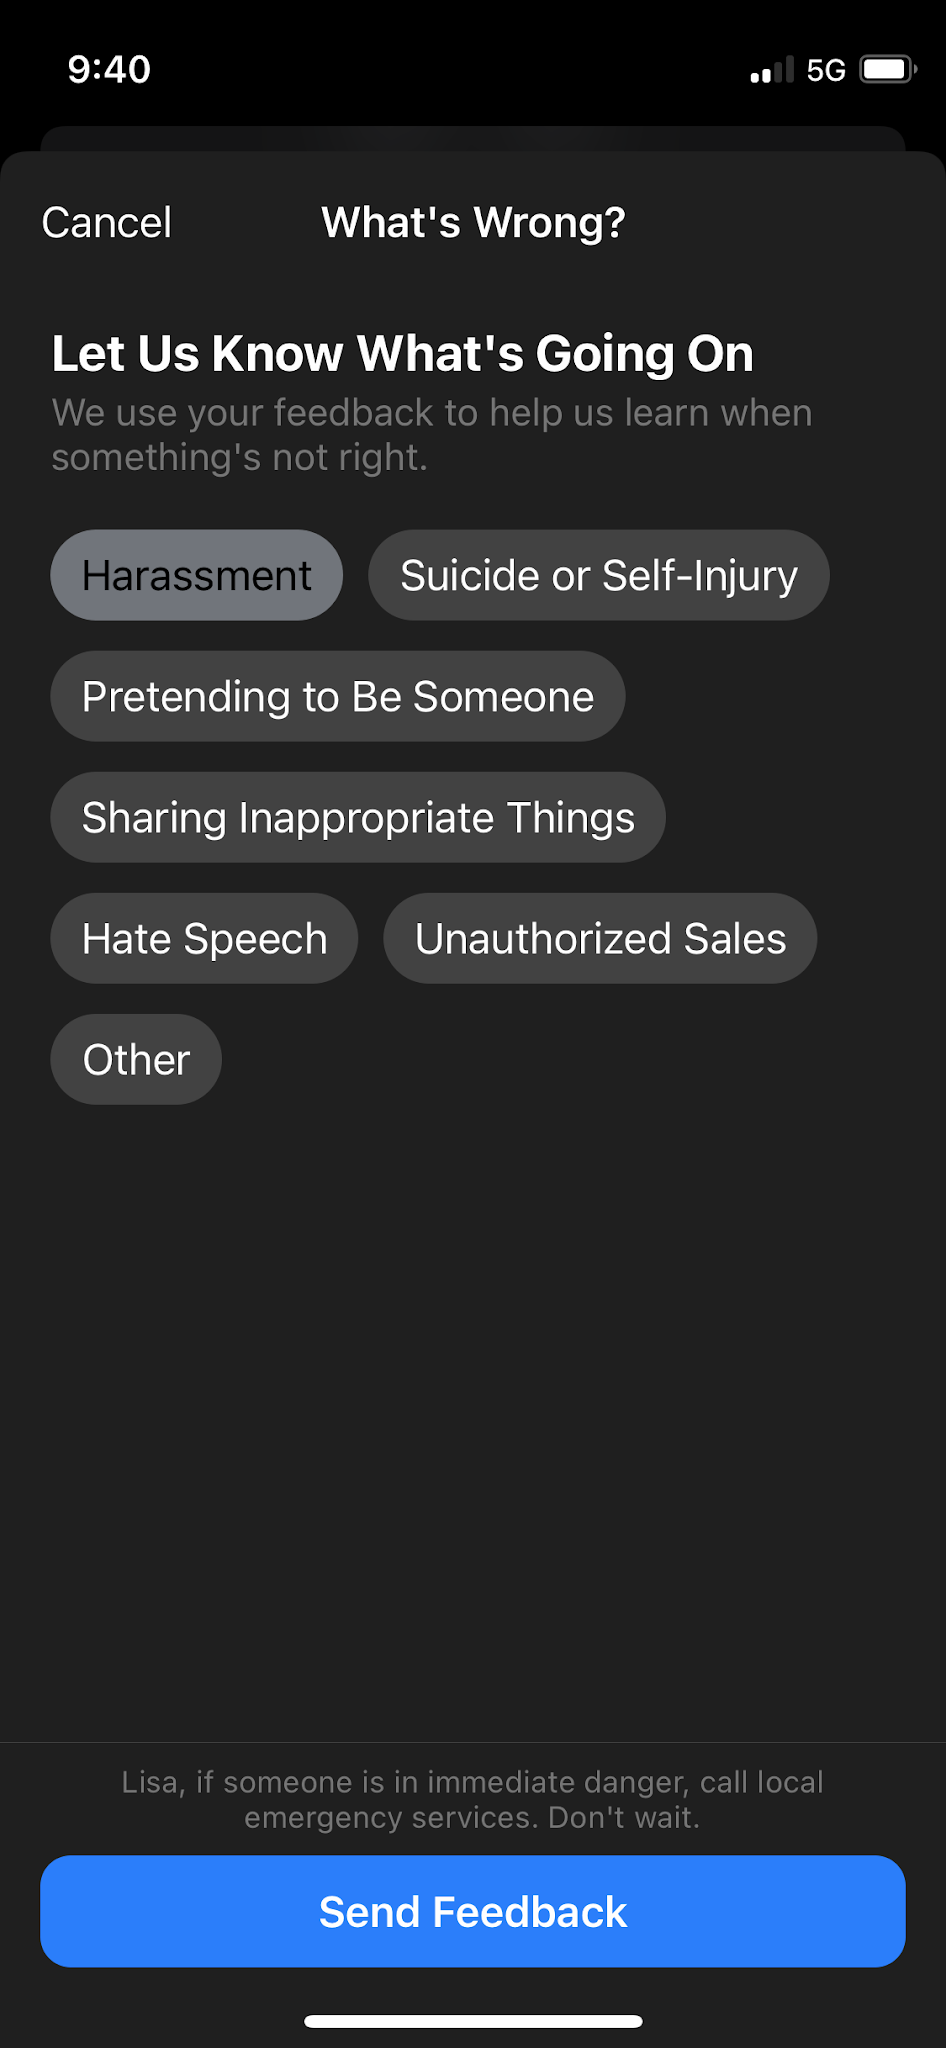
\includegraphics[width=0.49\textwidth]{harassment-reporting-example}
    \end{columns}
\end{frame}

\begin{frame}{Shadow Blocking}
    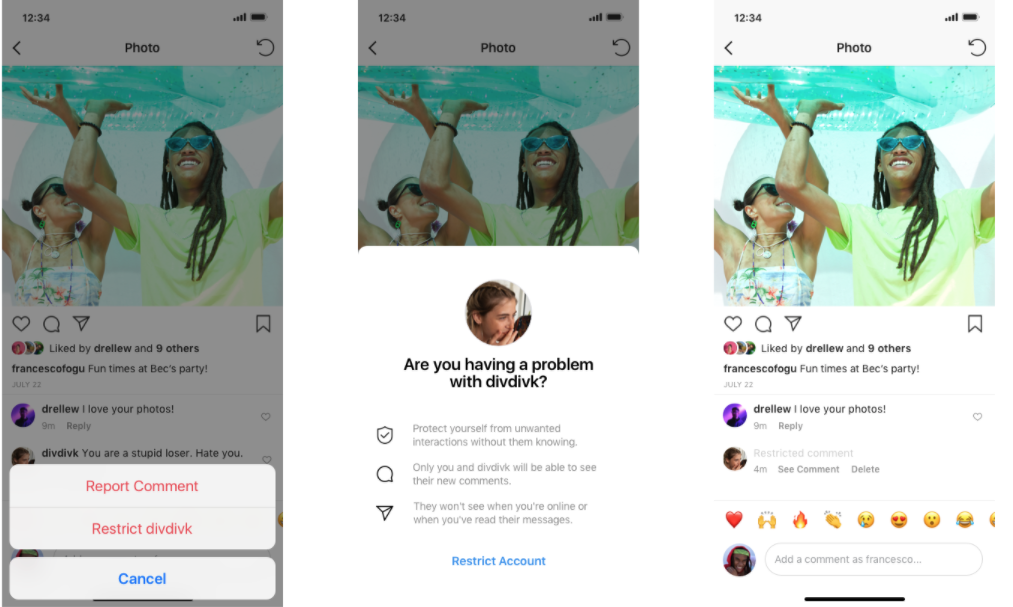
\includegraphics[width=\textwidth]{shadow-blocking}
\end{frame}

\begin{frame}{Platforms: Proactive Monitoring}
    \begin{columns}
        \column{0.55\textwidth}
            
\includegraphics[width=\textwidth]{false-positive-1}
            \begin{itemize}
                \item Recognizing sarcasm, joyful playing and culturally specific use of certain words/phrases can be hard for ML
                \item Important signals: 
                \begin{itemize}
                    \item Overall user karma
                    \begin{itemize}
                        \item How many people have blocked?
                        \item How often contacting strangers?
                    \end{itemize}
                    \item Relationship between sender and receiver
                \end{itemize}
            \end{itemize}
        \column{0.45\textwidth}
            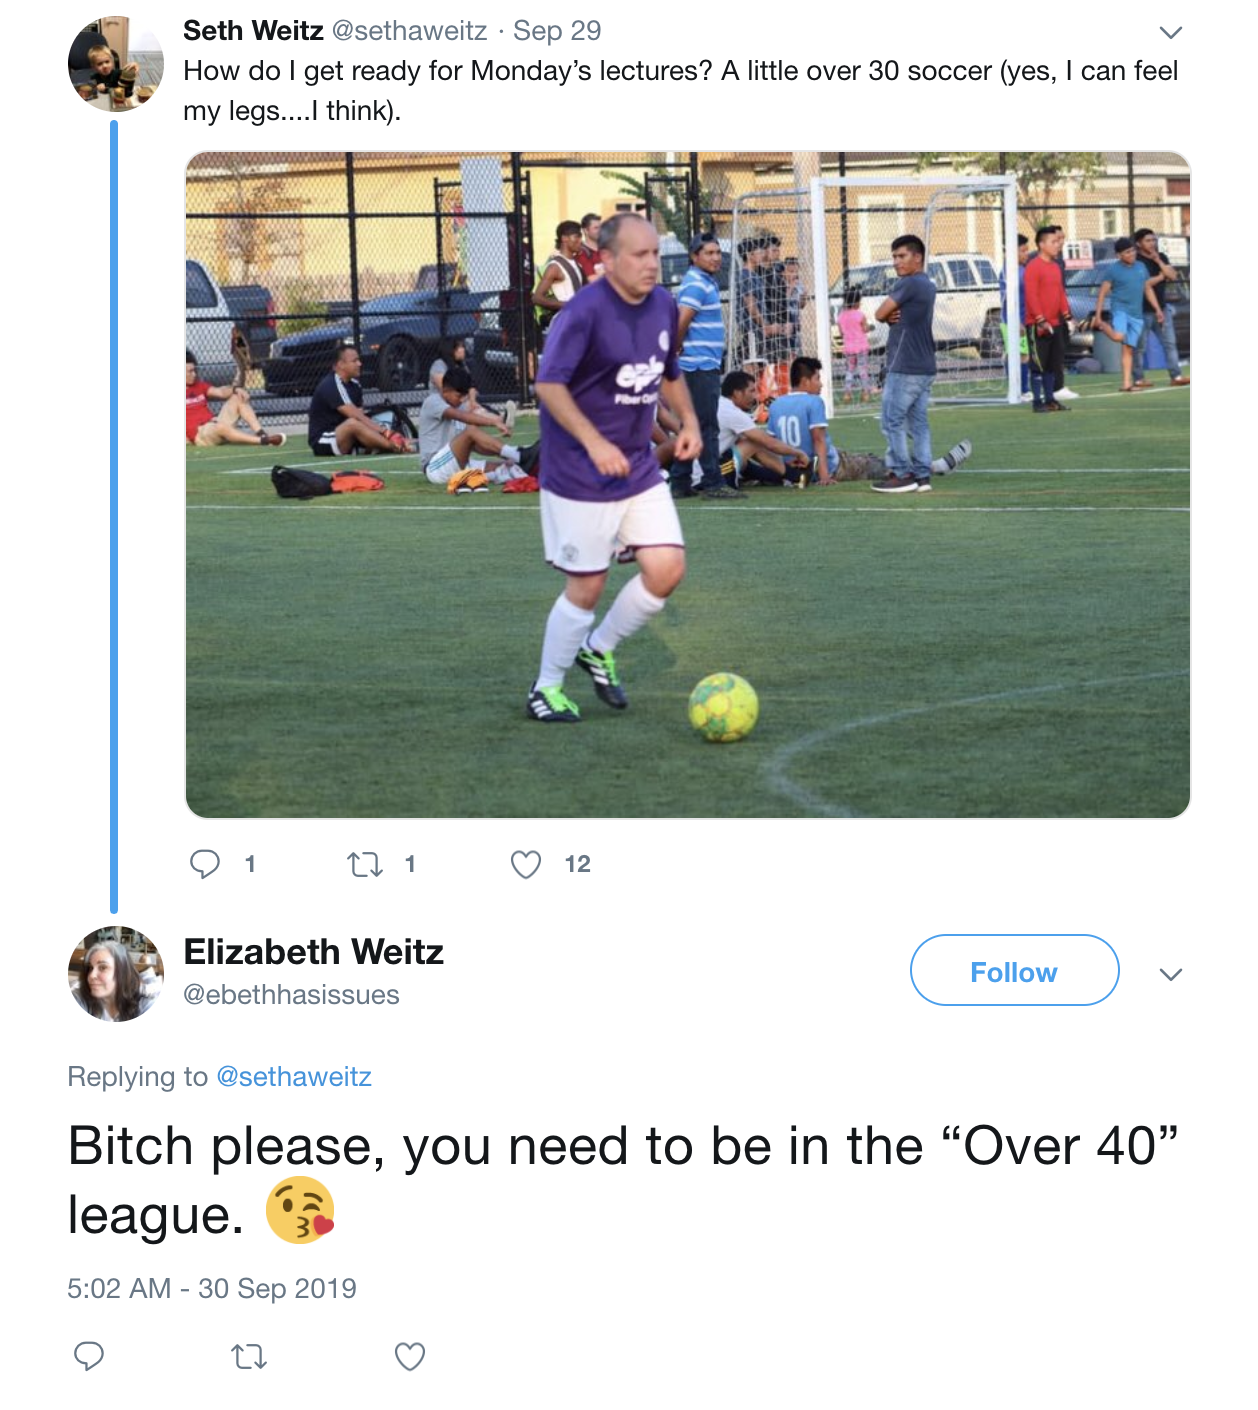
\includegraphics[width=\textwidth]{false-positive-2}
    \end{columns}
\end{frame}

\begin{frame}{Platforms: Productive Friction}
    \begin{columns}
        \column{0.35\textwidth}
            \small
            How can you build features into platforms to make it “more work” or “less fun” for harassers?
            \begin{itemize}
                \item Instagram: Restrict feature, where users block abusers and the abusers aren’t notified
                \item Instagram: Rethink feature, asking users to pause before posting material meeting AI patterns for bullying
            \end{itemize}
        \column{0.65\textwidth}
            
\includegraphics[width=\textwidth]{you-shall-not-pass}
    \end{columns}
\end{frame}

\begin{frame}{Third-Party Tools}
    
\includegraphics[width=\textwidth]{block-party}
    \begin{columns}[T]
        \column{0.45\textwidth}
            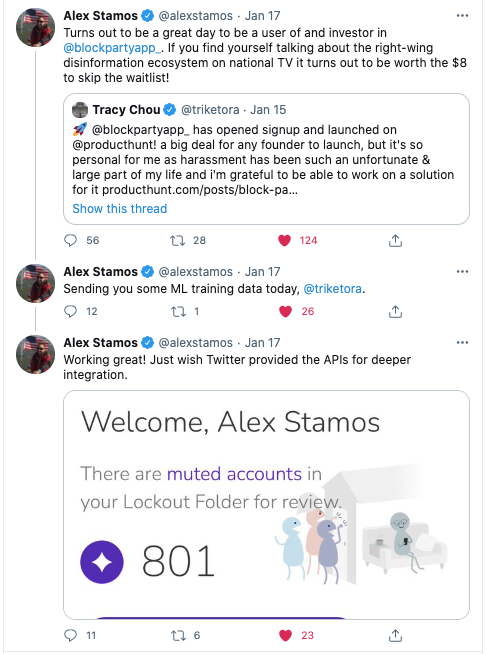
\includegraphics[width=\textwidth]{block-party-stamos-tweets}
        \column{0.4\textwidth}
            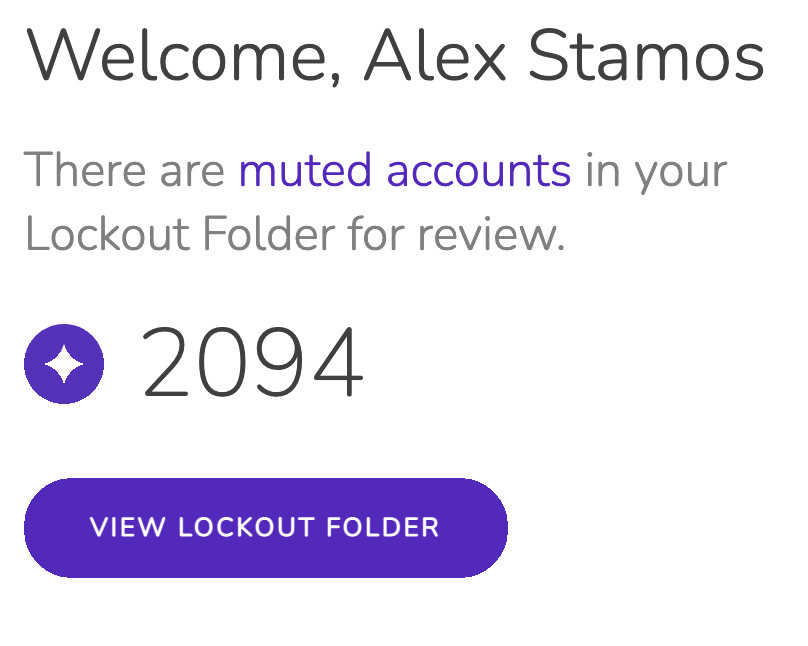
\includegraphics[width=\textwidth]{block-party-2}
            Disclaimer: I am an early investor in Block Party
    \end{columns}
\end{frame}

\begin{frame}{Third-Party Tools}
    \begin{columns}
        \column{0.5\textwidth}
            \includegraphics[width=\textwidth]{blocked-by-stamos}
            \includegraphics[width=\textwidth]{blocked-by-stamos-3}
        \column{0.5\textwidth}
            \includegraphics[width=\textwidth]{blocked-by-stamos-2}
            \includegraphics[width=\textwidth]{deleted-harassment-tweet}
    \end{columns}
\end{frame}

\begin{frame}{Privacy/Response Controls}
    \centering
    \includegraphics[width=0.45\textwidth]{greenwald-tweets}
\end{frame}

\section{Where Is This Going?}

\begin{frame}{Future: Harassment and E2EE}
    \begin{columns}
        \column{0.5\textwidth}
            \includegraphics[width=\textwidth]{signal}
        \column{0.5\textwidth}
            \begin{itemize}
                \item Like with all abuse, there is a hard safety-privacy trade-off
                \begin{itemize}
                    \item You can’t moderate what you can’t see
                \end{itemize}
                \item Options for private reporting exist
                \begin{itemize}
                    \item How much data is exposed?
                    \item Is one party consent ok?
                \end{itemize}
                \item Client-side ML is another area for focus
                \item Message Franking
            \end{itemize}
    \end{columns}
\end{frame}

\begin{frame}{Future: Coordination?}
    \begin{itemize}
        \item Currently, cross-platform coordination on counterterrorism and child sexual abuse.
        \item A centralized reporting service alerting platforms of coordinated harassment efforts?
        \item Downside: content cartels and standardization of speech
        \begin{itemize}
            \item Is it worth it?
        \end{itemize}
    \end{itemize}
    \includegraphics[width=\textwidth]{gifct}
\end{frame}

\end{document}